\subsection{\nogloxy{Premi::Back-End}}
\label{\nogloxy{Premi::Back-End}}
\subsubsection{Informazioni generali}
\begin{figure}[h]
\centering
\nogloxy{\includegraphics[scale=0.4,keepaspectratio]{diagrammi/package/{backEnd}.pdf}}
\caption{\nogloxy{Premi::Back-End}}
\end{figure}
\FloatBarrier
\begin{itemize}
\item \textbf{Descrizione}\\
Package contenente le componenti della parte \gloxy{back-end} dell'applicazione.
\item \textbf{Package contenuti}:
\begin{itemize}
\item \hyperref[\nogloxy{Premi::Back-End::App}]{\nogloxy{\texttt{App}}}\\
Package contenente le componenti del \gloxy{server} che implementano il pattern \gloxy{MVC}.
\item \hyperref[\nogloxy{Premi::Back-End::Config}]{\nogloxy{\texttt{Config}}}\\
Package contenente le componenti di configurazione del \gloxy{server}.
\end{itemize}
\end{itemize}
\subsubsection{Classi}
\subsubsubsection{\nogloxy{Premi::Back-End::Server}}
\label{\nogloxy{Premi::Back-End::Server}}
\begin{figure}[h]
\centering
\nogloxy{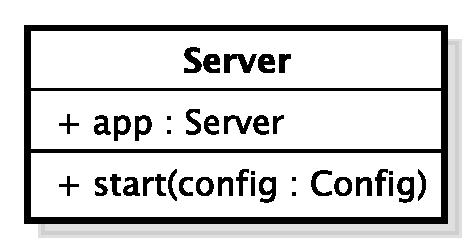
\includegraphics[scale=0.4,keepaspectratio]{diagrammi/classi/{BackEnd/server}.pdf}}
\caption{\nogloxy{Premi::Back-End::Server}}
\end{figure}
\FloatBarrier
\begin{itemize}
\item \textbf{Descrizione}\\
Classe che avvia il \gloxy{server}. Nello specifico apre una connessione al database tramite \gloxy{Mongoose}, invoca il middleware Express passando un riferimento al database \gloxy{MongoDB} come parametro in modo che possa configurarsi con esso, invoca il middleware Passport ed infine si mette in ascolto su una determinata porta. \`E il componente \gloxy{client} del \gloxy{design pattern} Chain of responsibility. Utilizza i moduli \gloxy{Mongoose}, Express, Passport e Chalk, quest’ultimo serve per definire lo stile dei tipi \texttt{String}.
\item \textbf{Utilizzo}\\
Utilizzato per avviare l’applicazione lato \gloxy{server}. Inizializza, internamente al \gloxy{back-end}, la catena di gestione delle chiamate \gloxy{REST} utilizzando le classi contenute nel package \texttt{Routers}.
\item \textbf{Relazioni con altre classi}:
\begin{itemize}
\item \textit{OUT} \hyperref[\nogloxy{Premi::Back-End::App::Routers::ProjectRouter}]{\nogloxy{\texttt{ProjectRouter}}}\\
Classe che gestisce le richieste relative alle operazioni riguardanti la mappa.  Componente ConcreteHandler del \gloxy{design pattern} Chain of responsibility.
\item \textit{OUT} \hyperref[\nogloxy{Premi::Back-End::App::Routers::StaticRouter}]{\nogloxy{\texttt{StaticRouter}}}\\
Classe che gestisce le richieste relative alle pagine statiche della componente \gloxy{back-end}. Componente ConcreteHandler del \gloxy{design pattern} Chain of responsibility.
\item \textit{OUT} \hyperref[\nogloxy{Premi::Back-End::App::Routers::UserRouter}]{\nogloxy{\texttt{UserRouter}}}\\
Classe che gestisce le richieste relative alla registrazione e alla gestione della sessione di un utente. Componente ConcreteHandler del \gloxy{design pattern} Chain of responsibility. Utilizza il modulo Passport.
\item \textit{OUT} \hyperref[\nogloxy{Premi::Back-End::Config::Config}]{\nogloxy{\texttt{Config}}}\\
Questa classe gestisce la configurazione del \gloxy{server}. \textit{Non sono stati modellati attributi e metodi di questa classe in quanto viene gestita da Express.}
\end{itemize}
\item \textbf{Attributi}:
\begin{itemize}
\item \nogloxy{\texttt{+ app: Server}}
\\ Espone l'istanza di Express che rappresenta l'applicazione lato \gloxy{server}.
\end{itemize}
\item \textbf{Metodi}:
\begin{itemize}
\item \nogloxy{\texttt{+ start(config: Config)}}
\\ Avvia il \gloxy{server} sfruttando i parametri di configurazione contenuti nell'oggetto \texttt{config}.
\\ \textbf{Parametri}:
\begin{itemize}
\item \nogloxy{\texttt{config: Config}}
\\ Rappresenta l'oggetto che contiene i dati di configurazione dell'applicazione.
\end{itemize}
\end{itemize}
\end{itemize}
\subsection{\nogloxy{Premi::Back-End::App}}
\label{\nogloxy{Premi::Back-End::App}}
\subsubsection{Informazioni generali}
\begin{figure}[h]
\centering
\nogloxy{\includegraphics[scale=0.4,keepaspectratio]{diagrammi/package/{backEnd-app}.pdf}}
\caption{\nogloxy{Premi::Back-End::App}}
\end{figure}
\FloatBarrier
\begin{itemize}
\item \textbf{Descrizione}\\
Package contenente le componenti del \gloxy{server} che implementano il pattern \gloxy{MVC}.
\item \textbf{Padre}: \hyperref[\nogloxy{Premi::Back-End}]{\nogloxy{\texttt{Back-End}}}
\item \textbf{Interazioni con altri componenti}:
\begin{itemize}
\item \hyperref[\nogloxy{Premi::Back-End::Config}]{\nogloxy{\texttt{Config}}}\\
Package contenente le componenti di configurazione del \gloxy{server}.
\end{itemize}
\item \textbf{Package contenuti}:
\begin{itemize}
\item \hyperref[\nogloxy{Premi::Back-End::App::Controllers}]{\nogloxy{\texttt{Controllers}}}\\
Package che contiene i controllers di Express, definisce la logica dell'applicazione.
\item \hyperref[\nogloxy{Premi::Back-End::App::Models}]{\nogloxy{\texttt{Models}}}\\
Package contenente le classi che definiscono il model dell'applicazione. Queste classi sono definite come classi schema di \gloxy{Mongoose}, il quale permette di utilizzare \gloxy{MongoDB} tramite degli oggetti.
\item \hyperref[\nogloxy{Premi::Back-End::App::Routers}]{\nogloxy{\texttt{Routers}}}\\
Package contenente i router della componente \gloxy{back-end} dell’applicazione. Contiene i file di configurazione relativi al routing delle richieste del \gloxy{client}, ossia i routes di Express.
\item \hyperref[\nogloxy{Premi::Back-End::App::Views}]{\nogloxy{\texttt{Views}}}\\
Package contenente le views della componente \gloxy{back-end} dell’applicazione.
\end{itemize}
\end{itemize}
\subsection{\nogloxy{Premi::Back-End::App::Controllers}}
\label{\nogloxy{Premi::Back-End::App::Controllers}}
\subsubsection{Informazioni generali}
\begin{figure}[h]
\centering
\nogloxy{\includegraphics[scale=0.4,keepaspectratio]{diagrammi/package/{backEnd-app-controllers}.pdf}}
\caption{\nogloxy{Premi::Back-End::App::Controllers}}
\end{figure}
\FloatBarrier
\begin{itemize}
\item \textbf{Descrizione}\\
Package che contiene i controllers di Express, definisce la logica dell'applicazione.
\item \textbf{Padre}: \hyperref[\nogloxy{Premi::Back-End::App}]{\nogloxy{\texttt{App}}}
\item \textbf{Interazioni con altri componenti}:
\begin{itemize}
\item \hyperref[\nogloxy{Premi::Back-End::App::Routers}]{\nogloxy{\texttt{Routers}}}\\
Package contenente i router della componente \gloxy{back-end} dell’applicazione. Contiene i file di configurazione relativi al routing delle richieste del \gloxy{client}, ossia i routes di Express.
\item \hyperref[\nogloxy{Premi::Back-End::App::Views}]{\nogloxy{\texttt{Views}}}\\
Package contenente le views della componente \gloxy{back-end} dell’applicazione.
\end{itemize}
\item \textbf{Package contenuti}:
\begin{itemize}
\item \hyperref[\nogloxy{Premi::Back-End::App::Controllers::Errors}]{\nogloxy{\texttt{Errors}}}\\
Package contenente i controllers per la gestione degli errori specifici.
\item \hyperref[\nogloxy{Premi::Back-End::App::Controllers::Projects}]{\nogloxy{\texttt{Projects}}}\\
Package contenente i controllers relativi alla gestione della mappa mentale.
\item \hyperref[\nogloxy{Premi::Back-End::App::Controllers::Users}]{\nogloxy{\texttt{Users}}}\\
Package contenente i controllers relativi alla gestione dell'autenticazione dell'utente.
\end{itemize}
\end{itemize}
\subsubsection{Classi}
\subsubsubsection{\nogloxy{Premi::Back-End::App::Controllers::ErrorHandler}}
\label{\nogloxy{Premi::Back-End::App::Controllers::ErrorHandler}}
\begin{figure}[h]
\centering
\nogloxy{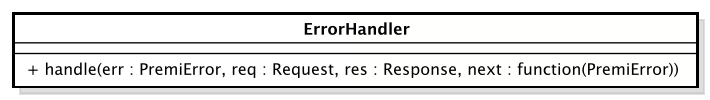
\includegraphics[scale=0.4,keepaspectratio]{diagrammi/classi/{BackEnd/App/Controllers/errorHandler}.pdf}}
\caption{\nogloxy{Premi::Back-End::App::Controllers::ErrorHandler}}
\end{figure}
\FloatBarrier
\begin{itemize}
\item \textbf{Descrizione}\\
Classe middleware per la gestione degli errori. Ritorna al \gloxy{client} un oggetto di tipo \texttt{Response} con stato HTTP 500 e descrizione dell'errore in formato \gloxy{JSON}. \`E un componente ConcreteHandler del \gloxy{design pattern} Chain of responsibility.
\item \textbf{Utilizzo}\\
Viene utilizzata quando si verifica un errore. Si preoccupa di delegare la costruzione del messaggio d’errore al modulo specifico qualora questo esista, altrimenti costruisce un messaggio d'errore generico.
In questo modo i messaggi d'errore specifici vengono delegati ad un altro modulo, rendendo così possibile aggiungere in futuro altri moduli per gestire più flessibilmente nuove tipologie di errori.
\item \textbf{Relazioni con altre classi}:
\begin{itemize}
\item \textit{IN} \hyperref[\nogloxy{Premi::Back-End::App::Routers::ProjectRouter}]{\nogloxy{\texttt{ProjectRouter}}}\\
Classe che gestisce le richieste relative alle operazioni riguardanti la mappa.  Componente ConcreteHandler del \gloxy{design pattern} Chain of responsibility.
\item \textit{IN} \hyperref[\nogloxy{Premi::Back-End::App::Routers::StaticRouter}]{\nogloxy{\texttt{StaticRouter}}}\\
Classe che gestisce le richieste relative alle pagine statiche della componente \gloxy{back-end}. Componente ConcreteHandler del \gloxy{design pattern} Chain of responsibility.
\item \textit{IN} \hyperref[\nogloxy{Premi::Back-End::App::Routers::UserRouter}]{\nogloxy{\texttt{UserRouter}}}\\
Classe che gestisce le richieste relative alla registrazione e alla gestione della sessione di un utente. Componente ConcreteHandler del \gloxy{design pattern} Chain of responsibility. Utilizza il modulo Passport.
\item \textit{OUT} \hyperref[\nogloxy{Premi::Back-End::App::Controllers::Errors::PremiError}]{\nogloxy{\texttt{PremiError}}}\\
Classe di gestione degli errori. Esegue la costruzione del messaggio d’errore specifico per i moduli di \texttt{Premi::Back-End::App}.
\end{itemize}
\item \textbf{Metodi}:
\begin{itemize}
\item \nogloxy{\texttt{+ handle(err: PremiError, req: Request, res: Response, next: function(PremiError))}}
\\ Metodo che gestisce la costruzione dei messaggi d’errore ritornando un \gloxy{JSON} contenente il messaggio d'errore.
\\ \textbf{Parametri}:
\begin{itemize}
\item \nogloxy{\texttt{err: PremiError}}
\\ Rappresenta l'errore di tipo \texttt{PremiError}.
\item \nogloxy{\texttt{req: Request}}
\\ Rappresenta la richiesta inviata al \gloxy{server}.
\item \nogloxy{\texttt{res: Response}}
\\ Rappresenta la risposta che il \gloxy{server} fornirà al termine dell’esecuzione del metodo.
\item \nogloxy{\texttt{next: function(PremiError)}}
\\ \dpNext
\end{itemize}
\end{itemize}
\end{itemize}
\subsubsubsection{\nogloxy{Premi::Back-End::App::Controllers::NotFoundHandler}}
\label{\nogloxy{Premi::Back-End::App::Controllers::NotFoundHandler}}
\begin{figure}[h]
\centering
\nogloxy{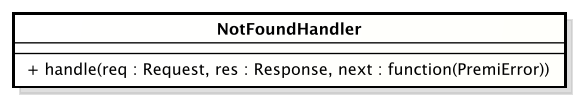
\includegraphics[scale=0.4,keepaspectratio]{diagrammi/classi/{BackEnd/App/Controllers/notFoundHandler}.pdf}}
\caption{\nogloxy{Premi::Back-End::App::Controllers::NotFoundHandler}}
\end{figure}
\FloatBarrier
\begin{itemize}
\item \textbf{Descrizione}\\
Classe che si occupa della gestione dell'errore di pagina non trovata. Componente
ConcreteHandler del \gloxy{design pattern} Chain of responsibility.
\item \textbf{Utilizzo}\\
Viene utilizzata per generare una pagina 404 di errore nel caso in cui l'URI passato non corrisponda ad una risorsa presente nell'applicazione.
\item \textbf{Relazioni con altre classi}:
\begin{itemize}
\item \textit{IN} \hyperref[\nogloxy{Premi::Back-End::App::Routers::ProjectRouter}]{\nogloxy{\texttt{ProjectRouter}}}\\
Classe che gestisce le richieste relative alle operazioni riguardanti la mappa.  Componente ConcreteHandler del \gloxy{design pattern} Chain of responsibility.
\item \textit{IN} \hyperref[\nogloxy{Premi::Back-End::App::Routers::StaticRouter}]{\nogloxy{\texttt{StaticRouter}}}\\
Classe che gestisce le richieste relative alle pagine statiche della componente \gloxy{back-end}. Componente ConcreteHandler del \gloxy{design pattern} Chain of responsibility.
\item \textit{IN} \hyperref[\nogloxy{Premi::Back-End::App::Routers::UserRouter}]{\nogloxy{\texttt{UserRouter}}}\\
Classe che gestisce le richieste relative alla registrazione e alla gestione della sessione di un utente. Componente ConcreteHandler del \gloxy{design pattern} Chain of responsibility. Utilizza il modulo Passport.
\end{itemize}
\item \textbf{Metodi}:
\begin{itemize}
\item \nogloxy{\texttt{+ handle(req: Request, res: Response)}}
\\ Metodo che gestisce la costruzione dei messaggi d’errore ritornando un \gloxy{JSON} contenente il messaggio d'errore.
\\ \textbf{Parametri}:
\begin{itemize}
\item \nogloxy{\texttt{req: Request}}
\\ Rappresenta la richiesta inviata al \gloxy{server}.
\item \nogloxy{\texttt{res: Response}}
\\ Rappresenta la risposta che il \gloxy{server} fornirà al termine dell’esecuzione del metodo.
\end{itemize}
\end{itemize}
\end{itemize}
\subsubsubsection{\nogloxy{Premi::Back-End::App::Controllers::ProjectController}}
\label{\nogloxy{Premi::Back-End::App::Controllers::ProjectController}}
\begin{figure}[h]
\centering
\nogloxy{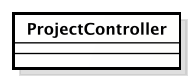
\includegraphics[scale=0.4,keepaspectratio]{diagrammi/classi/{BackEnd/App/Controllers/projectController}.pdf}}
\caption{\nogloxy{Premi::Back-End::App::Controllers::ProjectController}}
\end{figure}
\FloatBarrier
\begin{itemize}
\item \textbf{Descrizione}\\
Classe che raggruppa i vari controllers responsabili delle operazioni riguardanti la \gloxy{mappa mentale} attraverso \texttt{require}.
\item \textbf{Utilizzo}\\
Viene utilizzata per raggruppare i controllers responsabili della \gloxy{mappa mentale} in modo da rendere più pulito il codice delle classi che utilizzano tali controllers. In questo modo le classi che vogliono comunicare con i controllers della \gloxy{mappa mentale} necessitano di includere solo questa classe e non ogni singolo \gloxy{controller}.
\item \textbf{Relazioni con altre classi}:
\begin{itemize}
\item \textit{IN} \hyperref[\nogloxy{Premi::Back-End::App::Routers::ProjectRouter}]{\nogloxy{\texttt{ProjectRouter}}}\\
Classe che gestisce le richieste relative alle operazioni riguardanti la mappa.  Componente ConcreteHandler del \gloxy{design pattern} Chain of responsibility.
\item \textit{OUT} \hyperref[\nogloxy{Premi::Back-End::App::Controllers::Projects::NodeController}]{\nogloxy{\texttt{NodeController}}}\\
Classe che gestisce la logica applicativa riguardante la visualizzazione e la modifica dei nodi presenti in un \gloxy{progetto}.
\item \textit{OUT} \hyperref[\nogloxy{Premi::Back-End::App::Controllers::Projects::PathController}]{\nogloxy{\texttt{PathController}}}\\
Classe che gestisce la logica applicativa riguardante la visualizzazione e la modifica dei \gloxy{percorsi di presentazione} di un \gloxy{progetto}.
\item \textit{OUT} \hyperref[\nogloxy{Premi::Back-End::App::Controllers::Projects::ProjectManagementController}]{\nogloxy{\texttt{ProjectManagementController}}}\\
Classe che gestisce la logica applicativa riguardante la visualizzazione e la modifica dei \gloxy{progetti}. Rappresenta il ConcreteHandler nel \gloxy{design pattern} Chain of responsibility. Utilizza Passport.
\end{itemize}
\end{itemize}
\subsubsubsection{\nogloxy{Premi::Back-End::App::Controllers::StaticController}}
\label{\nogloxy{Premi::Back-End::App::Controllers::StaticController}}
\begin{figure}[h]
\centering
\nogloxy{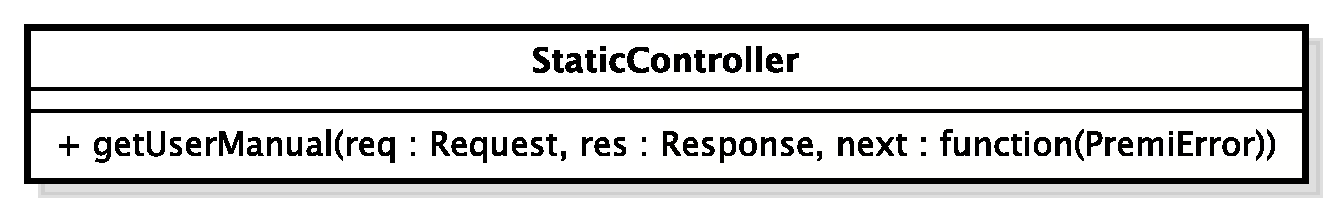
\includegraphics[scale=0.4,keepaspectratio]{diagrammi/classi/{BackEnd/App/Controllers/staticController}.pdf}}
\caption{\nogloxy{Premi::Back-End::App::Controllers::StaticController}}
\end{figure}
\FloatBarrier
\begin{itemize}
\item \textbf{Descrizione}\\
Classe che gestisce le operazioni e la logica applicativa riguardante la visualizzazione di pagine \gloxy{HTML} statiche. Rappresenta uno dei componenti ConcreteHandler del \gloxy{design pattern} Chain of responsibility.
\item \textbf{Utilizzo}\\
Viene utilizzata per gestire la visualizzazione di pagine \gloxy{HTML} statiche come il manuale utente.
\item \textbf{Relazioni con altre classi}:
\begin{itemize}
\item \textit{IN} \hyperref[\nogloxy{Premi::Back-End::App::Routers::StaticRouter}]{\nogloxy{\texttt{StaticRouter}}}\\
Classe che gestisce le richieste relative alle pagine statiche della componente \gloxy{back-end}. Componente ConcreteHandler del \gloxy{design pattern} Chain of responsibility.
\item \textit{OUT} \hyperref[\nogloxy{Premi::Back-End::App::Views::UserManualView}]{\nogloxy{\texttt{UserManualView}}}\\
Pagina \gloxy{HTML} statica contenente il manuale dell’applicazione.
\end{itemize}
\item \textbf{Metodi}:
\begin{itemize}
\item \nogloxy{\texttt{+ getUserManual(req: Request, res: Response)}}
\\ Si occupa di restituire, attraverso il parametro \texttt{res}, la pagina del manuale utente richiesta dal \gloxy{client}.
\\ \textbf{Parametri}:
\begin{itemize}
\item \nogloxy{\texttt{req: Request}}
\\ Rappresenta la richiesta inviata dal \gloxy{client}
\item \nogloxy{\texttt{res: Response}}
\\ Rappresenta la risposta che il \gloxy{server} fornirà al termine dell’esecuzione del metodo.
\end{itemize}
\end{itemize}
\end{itemize}
\subsubsubsection{\nogloxy{Premi::Back-End::App::Controllers::UserController}}
\label{\nogloxy{Premi::Back-End::App::Controllers::UserController}}
\begin{figure}[h]
\centering
\nogloxy{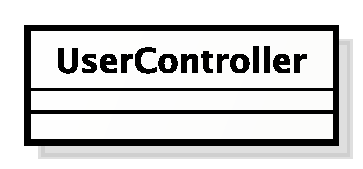
\includegraphics[scale=0.4,keepaspectratio]{diagrammi/classi/{BackEnd/App/Controllers/userController}.pdf}}
\caption{\nogloxy{Premi::Back-End::App::Controllers::UserController}}
\end{figure}
\FloatBarrier
\begin{itemize}
\item \textbf{Descrizione}\\
Classe che raggruppa attraverso \texttt{require} i vari controllers responsabili delle operazioni legate alla gestione degli utenti.
Si è scelto di predisporre questo raggruppamento per facilitare l’introduzione di nuove funzionalità legate alla gestione degli utenti.
\item \textbf{Utilizzo}\\
Viene utilizzata per raggruppare i controllers responsabili della gestione dei dati degli utenti. In questo modo le classi che vogliono comunicare con i controllers legati agli utenti necessitano di includere solo questa classe e non ogni singolo \gloxy{controller}.
\item \textbf{Relazioni con altre classi}:
\begin{itemize}
\item \textit{IN} \hyperref[\nogloxy{Premi::Back-End::App::Routers::UserRouter}]{\nogloxy{\texttt{UserRouter}}}\\
Classe che gestisce le richieste relative alla registrazione e alla gestione della sessione di un utente. Componente ConcreteHandler del \gloxy{design pattern} Chain of responsibility. Utilizza il modulo Passport.
\item \textit{OUT} \hyperref[\nogloxy{Premi::Back-End::App::Controllers::Users::AuthenticationController}]{\nogloxy{\texttt{AuthenticationController}}}\\
Classe che si occupa della registrazione e dell’autenticazione dell’utente nel sistema. \`E un componente ConcreteHandler del \gloxy{design pattern} Chain of responsibility. Risulta essere il componente che eventualmente esegue la richiesta del \gloxy{client} attraverso Passport.
\item \textit{OUT} \hyperref[\nogloxy{Premi::Back-End::App::Controllers::Users::AuthorizationController}]{\nogloxy{\texttt{AuthorizationController}}}\\
Classe middleware che, utilizzando Passport, si occupa di controllare la consistenza dell'oggetto \texttt{session} durante la sessione associata all'utente autenticato.  \`E un componente ConcreteHandler del \gloxy{design pattern} Chain of responsibility.
\end{itemize}
\end{itemize}
\subsection{\nogloxy{Premi::Back-End::App::Controllers::Errors}}
\label{\nogloxy{Premi::Back-End::App::Controllers::Errors}}
\subsubsection{Informazioni generali}
\begin{figure}[h]
\centering
\nogloxy{\includegraphics[scale=0.4,keepaspectratio]{diagrammi/package/{backEnd-app-controllers-errors}.pdf}}
\caption{\nogloxy{Premi::Back-End::App::Controllers::Errors}}
\end{figure}
\FloatBarrier
\begin{itemize}
\item \textbf{Descrizione}\\
Package contenente i controllers per la gestione degli errori specifici.
\item \textbf{Padre}: \hyperref[\nogloxy{Premi::Back-End::App::Controllers}]{\nogloxy{\texttt{Controllers}}}
\end{itemize}
\subsubsection{Classi}
\subsubsubsection{\nogloxy{Premi::Back-End::App::Controllers::Errors::PremiError}}
\label{\nogloxy{Premi::Back-End::App::Controllers::Errors::PremiError}}
\begin{figure}[h]
\centering
\nogloxy{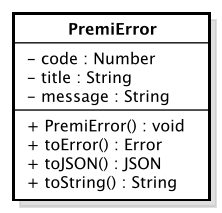
\includegraphics[scale=0.4,keepaspectratio]{diagrammi/classi/{BackEnd/App/Controllers/Errors/premiError}.pdf}}
\caption{\nogloxy{Premi::Back-End::App::Controllers::Errors::PremiError}}
\end{figure}
\FloatBarrier
\begin{itemize}
\item \textbf{Descrizione}\\
Classe di gestione degli errori. Esegue la costruzione del messaggio d’errore specifico per i moduli di \texttt{Premi::Back-End::App}.
\item \textbf{Utilizzo}\\
Viene utilizzato da ErrorsHandler quando si verifica un errore specifico relativo alle classi di \texttt{Premi::Back-End::App}.
\item \textbf{Relazioni con altre classi}:
\begin{itemize}
\item \textit{IN} \hyperref[\nogloxy{Premi::Back-End::App::Controllers::ErrorHandler}]{\nogloxy{\texttt{ErrorHandler}}}\\
Classe middleware per la gestione degli errori. Ritorna al \gloxy{client} un oggetto di tipo \texttt{Response} con stato HTTP 500 e descrizione dell'errore in formato \gloxy{JSON}. \`E un componente ConcreteHandler del \gloxy{design pattern} Chain of responsibility.
\end{itemize}
\item \textbf{Attributi}:
\begin{itemize}
\item \nogloxy{\texttt{- code: Number}}
\\ Campo dati contenente il codice dell'errore.
\item \nogloxy{\texttt{- message: String}}
\\ Campo dati contenente il messaggio che corrisponde all'errore.
\item \nogloxy{\texttt{- title: String}}
\\ Campo dati contenente il titolo dell'errore in forma di stringa
\end{itemize}
\item \textbf{Metodi}:
\begin{itemize}
\item \nogloxy{\texttt{+ PremiError(err: Number)}}
\\ Costruttore della classe \texttt{PremiError}.
\\ \textbf{Parametri}:
\begin{itemize}
\item \nogloxy{\texttt{err: Number}}
\\ Rappresenta il codice identificativo dell'errore.
\end{itemize}
\item \nogloxy{\texttt{+ toJSON(): JSON}}
\\ Questo metodo ritorna l'errore in formato \gloxy{JSON}.
\item \nogloxy{\texttt{+ toString(): String}}
\\ Effettua una concatenazione dei campi dati dell'errore e li ritorna in formato \texttt{String}.
\end{itemize}
\end{itemize}
\subsection{\nogloxy{Premi::Back-End::App::Controllers::Projects}}
\label{\nogloxy{Premi::Back-End::App::Controllers::Projects}}
\subsubsection{Informazioni generali}
\begin{figure}[h]
\centering
\nogloxy{\includegraphics[scale=0.4,keepaspectratio]{diagrammi/package/{backEnd-app-controllers-projects}.pdf}}
\caption{\nogloxy{Premi::Back-End::App::Controllers::Projects}}
\end{figure}
\FloatBarrier
\begin{itemize}
\item \textbf{Descrizione}\\
Package contenente i controllers relativi alla gestione della mappa mentale.
\item \textbf{Padre}: \hyperref[\nogloxy{Premi::Back-End::App::Controllers}]{\nogloxy{\texttt{Controllers}}}
\end{itemize}
\subsubsection{Classi}
\subsubsubsection{\nogloxy{Premi::Back-End::App::Controllers::Projects::NodeController}}
\label{\nogloxy{Premi::Back-End::App::Controllers::Projects::NodeController}}
\begin{figure}[h]
\centering
\nogloxy{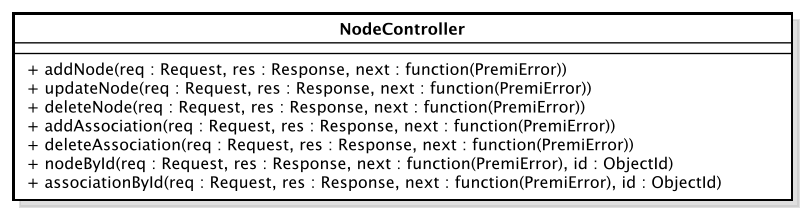
\includegraphics[scale=0.4,keepaspectratio]{diagrammi/classi/{BackEnd/App/Controllers/Projects/nodeController}.pdf}}
\caption{\nogloxy{Premi::Back-End::App::Controllers::Projects::NodeController}}
\end{figure}
\FloatBarrier
\begin{itemize}
\item \textbf{Descrizione}\\
Classe che gestisce la logica applicativa riguardante la visualizzazione e la modifica dei nodi presenti in un \gloxy{progetto}.
\item \textbf{Utilizzo}\\
Viene utilizzata per implementare le funzionalità necessarie a gestire le richieste \gloxy{REST} legate ai nodi presenti in un \gloxy{progetto}.
\item \textbf{Relazioni con altre classi}:
\begin{itemize}
\item \textit{IN} \hyperref[\nogloxy{Premi::Back-End::App::Controllers::ProjectController}]{\nogloxy{\texttt{ProjectController}}}\\
Classe che raggruppa i vari controllers responsabili delle operazioni riguardanti la \gloxy{mappa mentale} attraverso \texttt{require}.
\item \textit{OUT} \hyperref[\nogloxy{Premi::Back-End::App::Models::ProjectModel}]{\nogloxy{\texttt{ProjectModel}}}\\
Questa classe rappresenta una mappa mentale, che contiene nodi, relazioni tra i nodi e \gloxy{percorsi} di presentazione.
\end{itemize}
\item \textbf{Metodi}:
\begin{itemize}
\item \nogloxy{\texttt{+ addAssociation(req: Request, res: Response, next: function(PremiError))}}
\\ Aggiunge una relazione di tipo associazione tra due nodi presenti nella \gloxy{mappa mentale} del \gloxy{progetto} correntemente in uso dall’utente che ha effettuato il login.
\\ \textbf{Parametri}:
\begin{itemize}
\item \nogloxy{\texttt{req: Request}}
\\ Rappresenta la richiesta inviata al \gloxy{server}. Contiene l’identificativo dell’utente che ha effettuato la login. In \texttt{req} sono contenuti anche campi dati che rappresentano l’identificativo del \gloxy{progetto} nel database, l’identificativo del nodo sorgente della relazione e quello del nodo destinazione.
\item \nogloxy{\texttt{res: Response}}
\\ Rappresenta la risposta che il \gloxy{server} fornirà al termine dell’esecuzione del metodo.
\item \nogloxy{\texttt{next: function(PremiError)}}
\\ \dpNext
\end{itemize}
\item \nogloxy{\texttt{+ addNode(req: Request, res: Response, next: function(PremiError))}}
\\ Aggiunge un nuovo nodo vuoto alla \gloxy{mappa mentale} del \gloxy{progetto} correntemente in uso dall’utente autenticato, specificandone il collegamento con il nodo padre.
\\ \textbf{Parametri}:
\begin{itemize}
\item \nogloxy{\texttt{req: Request}}
\\ Rappresenta la richiesta inviata al \gloxy{server}. Contiene l’identificativo dell’utente che ha effettuato la login, l’identificativo del \gloxy{progetto} che sta modificando e l’identificativo del nodo di cui è figlio.
\item \nogloxy{\texttt{res: Response}}
\\ Rappresenta la risposta che il \gloxy{server} fornirà al termine dell’esecuzione del metodo.
\item \nogloxy{\texttt{next: function(PremiError)}}
\\ \dpNext
\end{itemize}
\item \nogloxy{\texttt{+ associationById(req: Request, res: Response, next: function(PremiError), id: ObjectId)}}
\\ Middleware sui parametri delle richieste \gloxy{REST} relative all'id dell'associazione logica(non gerarchica). Controlla che l'id dell'associazione esista nel database: se ciò è verificato passa il controllo al successivo ConcreteHandler, altrimenti passa il controllo alla catena di gestione degli errori.
\\ \textbf{Parametri}:
\begin{itemize}
\item \nogloxy{\texttt{req: Request}}
\\ Rappresenta la richiesta inviata al \gloxy{server}.
\item \nogloxy{\texttt{res: Response}}
\\ Rappresenta la risposta che fornirà il \gloxy{server}.
\item \nogloxy{\texttt{next: function(PremiError)}}
\\ \dpNext
\item \nogloxy{\texttt{id: ObjectId}}
\\ Rappresenta l'identificativo dell'associazione.
\end{itemize}
\item \nogloxy{\texttt{+ deleteAssociation(req: Request, res: Response, next: function(PremiError))}}
\\ Rimuove una relazione di tipo \texttt{association} tra due nodi presenti nella \gloxy{mappa mentale} del \gloxy{progetto} correntemente in uso dall’utente che ha effettuato il login.
\\ \textbf{Parametri}:
\begin{itemize}
\item \nogloxy{\texttt{req: Request}}
\\ \`E l’oggetto che rappresenta la richiesta inviata al \gloxy{server}. Il metodo legge l’identificativo dell’utente che ha effettuato la login. In \texttt{req} sono contenuti anche campi dati che rappresentano l’identificativo del \gloxy{progetto} nel database, l’identificativo del nodo sorgente della relazione e quello del nodo destinazione della relazione da eliminare.
\item \nogloxy{\texttt{res: Response}}
\\ \`E l’oggetto che rappresenta la risposta che il \gloxy{server} fornirà al termine dell’esecuzione del metodo.
\item \nogloxy{\texttt{next: function(PremiError)}}
\\ Questo parametro rappresenta la \gloxy{callback} che il metodo deve chiamare qualora si verificassero errori nell'esecuzione del metodo.
\end{itemize}
\item \nogloxy{\texttt{+ deleteNode(req: Request, res: Response, next: function(PremiError))}}
\\ Rimuove un nodo dalla \gloxy{mappa mentale} del \gloxy{progetto} correntemente in uso dall’utente che ha effettuato il login. Restituisce la mappa mentale, comprendente nodi e relazioni come un oggetto \gloxy{JSON}, priva del nodo rimosso e dell’eventuale sottoalbero di cui era padre.
\\ \textbf{Parametri}:
\begin{itemize}
\item \nogloxy{\texttt{req: Request}}
\\ Rappresenta la richiesta inviata al \gloxy{server}. Contiene l’identificativo dell’utente che ha effettuato la login, l’identificativo del \gloxy{progetto} che sta modificando e l’identificativo del nodo da rimuovere dalla mappa mentale.
\item \nogloxy{\texttt{res: Response}}
\\ Rappresenta la risposta che il \gloxy{server} fornirà al termine dell’esecuzione del metodo.
\item \nogloxy{\texttt{next: function(PremiError)}}
\\ \dpNext
\end{itemize}
\item \nogloxy{\texttt{+ nodeById(req: Request, res: Response, next: function(PremiError), id: ObjectId)}}
\\ Middleware sui parametri delle richieste \gloxy{REST} relative all'id del nodo. Controlla che l'id del nodo esista nel database: se ciò è verificato passa il controllo al successivo ConcreteHandler, altrimenti passa il controllo alla catena di gestione degli errori.
\\ \textbf{Parametri}:
\begin{itemize}
\item \nogloxy{\texttt{req: Request}}
\\ Rappresenta la richiesta inviata dal \gloxy{client}.
\item \nogloxy{\texttt{res: Response}}
\\ Rappresenta la risposta che fornirà il \gloxy{server}.
\item \nogloxy{\texttt{next: function(PremiError)}}
\\ \dpNext
\item \nogloxy{\texttt{id: ObjectId}}
\\ Rappresenta l'identificativo del nodo.
\end{itemize}
\item \nogloxy{\texttt{+ updateNode(req: Request, res: Response, next: function(PremiError))}}
\\ Modifica il contenuto di un nodo della \gloxy{mappa mentale} del \gloxy{progetto} correntemente in uso dall’utente autenticato.
\\ \textbf{Parametri}:
\begin{itemize}
\item \nogloxy{\texttt{req: Request}}
\\ Rappresenta la richiesta inviata al \gloxy{server}. Contiene l’identificativo dell’utente che ha effettuato la login. In \texttt{req} sono contenuti anche campi dati che rappresentano l’identificativo del \gloxy{progetto} nel database, del nodo che il metodo deve modificare ed un oggetto \gloxy{JSON} che raccoglie le modifiche da apportare al nodo.
\item \nogloxy{\texttt{res: Response}}
\\ Rappresenta la risposta che il \gloxy{server} fornirà al termine dell’esecuzione del metodo.
\item \nogloxy{\texttt{next: function(PremiError)}}
\\ \dpNext
\end{itemize}
\end{itemize}
\end{itemize}
\subsubsubsection{\nogloxy{Premi::Back-End::App::Controllers::Projects::PathController}}
\label{\nogloxy{Premi::Back-End::App::Controllers::Projects::PathController}}
\begin{figure}[h]
\centering
\nogloxy{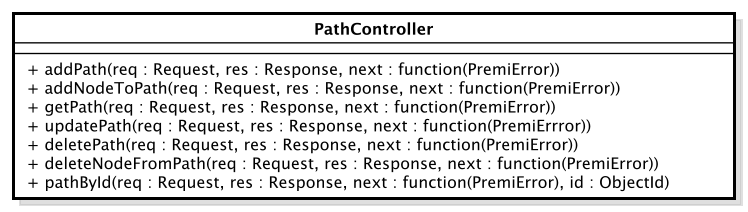
\includegraphics[scale=0.4,keepaspectratio]{diagrammi/classi/{BackEnd/App/Controllers/Projects/pathController}.pdf}}
\caption{\nogloxy{Premi::Back-End::App::Controllers::Projects::PathController}}
\end{figure}
\FloatBarrier
\begin{itemize}
\item \textbf{Descrizione}\\
Classe che gestisce la logica applicativa riguardante la visualizzazione e la modifica dei \gloxy{percorsi di presentazione} di un \gloxy{progetto}.
\item \textbf{Utilizzo}\\
Viene utilizzata per implementare le funzionalità necessarie a gestire le richieste \gloxy{REST} legate ai \gloxy{percorsi} di presentazione.
\item \textbf{Relazioni con altre classi}:
\begin{itemize}
\item \textit{IN} \hyperref[\nogloxy{Premi::Back-End::App::Controllers::ProjectController}]{\nogloxy{\texttt{ProjectController}}}\\
Classe che raggruppa i vari controllers responsabili delle operazioni riguardanti la \gloxy{mappa mentale} attraverso \texttt{require}.
\item \textit{OUT} \hyperref[\nogloxy{Premi::Back-End::App::Models::ProjectModel}]{\nogloxy{\texttt{ProjectModel}}}\\
Questa classe rappresenta una mappa mentale, che contiene nodi, relazioni tra i nodi e \gloxy{percorsi} di presentazione.
\end{itemize}
\item \textbf{Metodi}:
\begin{itemize}
\item \nogloxy{\texttt{+ addNodeToPath(req: Request, res: Response, next: function(PremiError))}}
\\ Aggiunge un nodo ad un \gloxy{percorso} del \gloxy{progetto} correntemente in uso dall’utente che ha effettuato il login.
\\ \textbf{Parametri}:
\begin{itemize}
\item \nogloxy{\texttt{req: Request}}
\\ Rappresenta la richiesta inviata al \gloxy{server}. Contiene l’identificativo dell’utente che ha effettuato la login, l’identificativo del \gloxy{progetto} che sta modificando, l’identificativo del \gloxy{percorso} da aggiornare e quello del nodo da inserire in esso.
\item \nogloxy{\texttt{res: Response}}
\\ Rappresenta la risposta che il \gloxy{server} fornirà al termine dell’esecuzione del metodo.
\item \nogloxy{\texttt{next: function(PremiError)}}
\\ \dpNext
\end{itemize}
\item \nogloxy{\texttt{+ addPath(req: Request, res: Response, next: function(PremiError))}}
\\ Crea un nuovo \gloxy{percorso} di presentazione, con un nome specificato nel parametro \texttt{req}. Restituisce un oggetto \gloxy{JSON} contenente l’identificativo, presente nel database, del \gloxy{percorso} creato.
\\ \textbf{Parametri}:
\begin{itemize}
\item \nogloxy{\texttt{req: Request}}
\\ Rappresenta la richiesta inviata al \gloxy{server}. Contiene l’identificativo dell’utente che ha effettuato la login, l’identificativo del \gloxy{progetto} che sta modificando e il nome del nuovo \gloxy{percorso} da inserire nel database.
\item \nogloxy{\texttt{res: Response}}
\\ Rappresenta la risposta che il \gloxy{server} fornirà al termine dell’esecuzione del metodo.
\item \nogloxy{\texttt{next: function(PremiError)}}
\\ \dpNext
\end{itemize}
\item \nogloxy{\texttt{+ deleteNodeFromPath(req: Request, res: Response, next: function(PremiError))}}
\\ Rimuove un nodo da un \gloxy{percorso} del \gloxy{progetto} correntemente in uso dall’utente che ha effettuato il login.
\\ \textbf{Parametri}:
\begin{itemize}
\item \nogloxy{\texttt{req: Request}}
\\ Rappresenta la richiesta inviata al \gloxy{server}. Contiene l’identificativo dell’utente che ha effettuato la login, l’identificativo del \gloxy{progetto} che sta modificando, l’identificativo del nodo da modificare e l’identificativo del nodo da rimuovere dal \gloxy{percorso}.
\item \nogloxy{\texttt{res: Response}}
\\ Rappresenta la risposta che il \gloxy{server} fornirà al termine dell’esecuzione del metodo.
\item \nogloxy{\texttt{next: function(PremiError)}}
\\ \dpNext
\end{itemize}
\item \nogloxy{\texttt{+ deletePath(req: Request, res: Response, next: function(PremiError))}}
\\ Elimina un \gloxy{percorso di presentazione} dal database.
\\ \textbf{Parametri}:
\begin{itemize}
\item \nogloxy{\texttt{req: Request}}
\\ Rappresenta la richiesta inviata al \gloxy{server}. Contiene l’identificativo dell’utente che ha effettuato la login, l’identificativo del \gloxy{progetto} che sta modificando e l’identificativo del \gloxy{percorso} da eliminare nel database.
\item \nogloxy{\texttt{res: Response}}
\\ Rappresenta la risposta che il \gloxy{server} fornirà al termine dell’esecuzione del metodo.
\item \nogloxy{\texttt{next: function(PremiError)}}
\\ \dpNext
\end{itemize}
\item \nogloxy{\texttt{+ getPath(req: Request, res: Response, next: function(PremiError))}}
\\ Restituisce un oggetto \gloxy{JSON} contenente tutti i nodi facenti parte di un \gloxy{percorso di presentazione} del \gloxy{progetto} correntemente in uso dall’utente che ha effettuato il login.
\\ \textbf{Parametri}:
\begin{itemize}
\item \nogloxy{\texttt{req: Request}}
\\ Rappresenta la richiesta inviata al \gloxy{server}. Contiene l’identificativo dell’utente che ha effettuato la login, l’identificativo del \gloxy{progetto} che sta modificando,  l’identificativo del \gloxy{percorso} di cui fornire l’insieme dei relativi nodi della mappa mentale.
\item \nogloxy{\texttt{res: Response}}
\\ Rappresenta la risposta che il \gloxy{server} fornirà al termine dell’esecuzione del metodo.
\item \nogloxy{\texttt{next: function(PremiError)}}
\\ \dpNext
\end{itemize}
\item \nogloxy{\texttt{+ pathById(req: Request, res: Response, next: function(PremiError), id: ObjectId)}}
\\ Middleware sui parametri delle richieste \gloxy{REST} relative all'id del path. Controlla che l'id del path esista nel database: se ciò è verificato passa il controllo al successivo ConcreteHandler, altrimenti passa il controllo alla catena di gestione degli errori.
\\ \textbf{Parametri}:
\begin{itemize}
\item \nogloxy{\texttt{req: Request}}
\\ Rappresenta la richiesta inviata dal \gloxy{client}.
\item \nogloxy{\texttt{res: Response}}
\\ Rappresenta la risposta che fornirà il \gloxy{server}.
\item \nogloxy{\texttt{next: function(PremiError)}}
\\ \dpNext
\item \nogloxy{\texttt{id: ObjectId}}
\\ Rappresenta l'identificativo del path.
\end{itemize}
\item \nogloxy{\texttt{+ updatePath(req: Request, res: Response, next: function(PremiError))}}
\\ Questo metodo viene utilizzato per modificare le impostazioni di un \gloxy{percorso di presentazione} nel database. In particolare è utilizzato per rinominare un \gloxy{percorso} di presentazione. Ottiene il nuovo nome dal parametro \texttt{req}. Restituisce un messaggio di conferma o un errore, nel formato \gloxy{JSON} stabilito.
\\ \textbf{Parametri}:
\begin{itemize}
\item \nogloxy{\texttt{req: Request}}
\\ Rappresenta la richiesta inviata al \gloxy{server}. Contiene legge l’identificativo dell’utente che ha effettuato la login, l’identificativo del \gloxy{progetto} che sta modificando, l’identificativo del \gloxy{percorso} di cui modificare il nome.
\item \nogloxy{\texttt{res: Response}}
\\ Rappresenta la risposta che il \gloxy{server} fornirà al termine dell’esecuzione del metodo.
\item \nogloxy{\texttt{next: function(PremiError)}}
\\ \dpNext
\end{itemize}
\end{itemize}
\end{itemize}
\subsubsubsection{\nogloxy{Premi::Back-End::App::Controllers::Projects::ProjectManagementController}}
\label{\nogloxy{Premi::Back-End::App::Controllers::Projects::ProjectManagementController}}
\begin{figure}[h]
\centering
\nogloxy{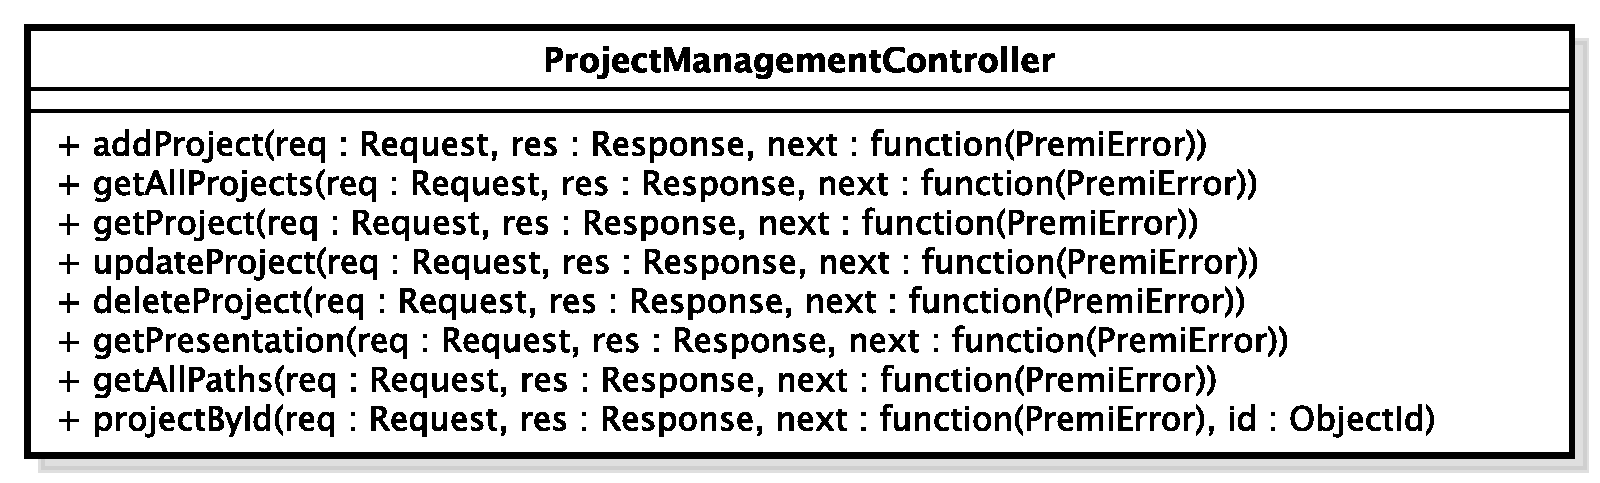
\includegraphics[scale=0.4,keepaspectratio]{diagrammi/classi/{BackEnd/App/Controllers/Projects/projectManagement}.pdf}}
\caption{\nogloxy{Premi::Back-End::App::Controllers::Projects::ProjectManagementController}}
\end{figure}
\FloatBarrier
\begin{itemize}
\item \textbf{Descrizione}\\
Classe che gestisce la logica applicativa riguardante la visualizzazione e la modifica dei \gloxy{progetti}. Rappresenta il ConcreteHandler nel \gloxy{design pattern} Chain of responsibility. Utilizza Passport.
\item \textbf{Utilizzo}\\
Viene utilizzata per implementare le funzionalità necessarie a gestire le richieste \gloxy{REST} legate ai \gloxy{progetti}.
\item \textbf{Relazioni con altre classi}:
\begin{itemize}
\item \textit{IN} \hyperref[\nogloxy{Premi::Back-End::App::Controllers::ProjectController}]{\nogloxy{\texttt{ProjectController}}}\\
Classe che raggruppa i vari controllers responsabili delle operazioni riguardanti la \gloxy{mappa mentale} attraverso \texttt{require}.
\item \textit{OUT} \hyperref[\nogloxy{Premi::Back-End::App::Models::ProjectModel}]{\nogloxy{\texttt{ProjectModel}}}\\
Questa classe rappresenta una mappa mentale, che contiene nodi, relazioni tra i nodi e \gloxy{percorsi} di presentazione.
\end{itemize}
\item \textbf{Metodi}:
\begin{itemize}
\item \nogloxy{\texttt{+ addProject(req: Request, res: Response, next: function(PremiError))}}
\\ Crea un nuovo \gloxy{progetto} associato all’utente autenticato.
\\ \textbf{Parametri}:
\begin{itemize}
\item \nogloxy{\texttt{req: Request}}
\\ Rappresenta la richiesta inviata al \gloxy{server}.
\item \nogloxy{\texttt{res: Response}}
\\ Rappresenta la risposta che il \gloxy{server} fornirà al termine dell’esecuzione del metodo.
\item \nogloxy{\texttt{next: function(PremiError)}}
\\ \dpNext
\end{itemize}
\item \nogloxy{\texttt{+ deleteProject(req: Request, res: Response, next: function(PremiError))}}
\\ Richiede al model la rimozione dal database di un \gloxy{progetto} associato all’utente autenticato.
\\ \textbf{Parametri}:
\begin{itemize}
\item \nogloxy{\texttt{req: Request}}
\\ Rappresenta la richiesta inviata al \gloxy{server}. Contiene l’identificativo dell’utente autenticato. In \texttt{req} è contenuto anche un campo che rappresenta l’identificativo del \gloxy{progetto} nel database che il metodo deve rimuovere.
\item \nogloxy{\texttt{res: Response}}
\\ Rappresenta la risposta che il \gloxy{server} fornirà al termine dell’esecuzione del metodo.
\item \nogloxy{\texttt{next: function(PremiError)}}
\\ \dpNext
\end{itemize}
\item \nogloxy{\texttt{+ getAllPaths(req: Request, res: Response, next: function(PremiError))}}
\\ Restituisce i \gloxy{percorsi di presentazione} del \gloxy{progetto} relativo all’utente della sessione. Altrimenti restituisce un messaggio di errore.
\\ \textbf{Parametri}:
\begin{itemize}
\item \nogloxy{\texttt{req: Request}}
\\ Rappresenta la richiesta inviata al \gloxy{server}.
\item \nogloxy{\texttt{res: Response}}
\\ Rappresenta la risposta che il \gloxy{server} fornirà al termine dell’esecuzione del metodo.
\item \nogloxy{\texttt{next: function(PremiError)}}
\\ \dpNext
\end{itemize}
\item \nogloxy{\texttt{+ getAllProjects(req: Request, res: Response, next: function(PremiError))}}
\\ Restituisce una lista contenente tutti i \gloxy{progetti} relativi all’utente autenticato, a cui vengono associati i \gloxy{percorsi di presentazione} creati, come un oggetto \gloxy{JSON}.
\\ \textbf{Parametri}:
\begin{itemize}
\item \nogloxy{\texttt{req: Request}}
\\ Rappresenta la richiesta inviata al \gloxy{server}. Contiene l’identificativo dell’utente autenticato.
\item \nogloxy{\texttt{res: Response}}
\\ Rappresenta la risposta che il \gloxy{server} fornirà al termine dell’esecuzione del metodo.
\item \nogloxy{\texttt{next: function(PremiError)}}
\\ \dpNext
\end{itemize}
\item \nogloxy{\texttt{+ getPresentation(req: Request, res: Response, next: function(PremiError))}}
\\ Questo metodo è utilizzato per fornire un oggetto \gloxy{JSON} contenente i nodi della \gloxy{mappa mentale} e le relazioni per il \gloxy{progetto} specificato. Indica inoltre quali nodi sono compresi nel \gloxy{percorso di presentazione} indicato.
\\ \textbf{Parametri}:
\begin{itemize}
\item \nogloxy{\texttt{req: Request}}
\\ Rappresenta la richiesta inviata al \gloxy{server}. Contiene l’identificativo dell’utente che ha effettuato la login e gli identificativi del \gloxy{progetto} e del \gloxy{percorso} di cui si vogliono ottenere i dati per la presentazione.
\item \nogloxy{\texttt{res: Response}}
\\ Rappresenta la risposta che il \gloxy{server} fornirà al termine dell’esecuzione del metodo.
\item \nogloxy{\texttt{next: function(PremiError)}}
\\ \dpNext
\end{itemize}
\item \nogloxy{\texttt{+ getProject(req: Request, res: Response, next: function(PremiError))}}
\\ Restituisce la \gloxy{mappa mentale} comprendente nodi e relazioni in formato \gloxy{JSON}. La \gloxy{mappa mentale} restituita è associata ad un \gloxy{progetto} dell’utente autenticato.
\\ \textbf{Parametri}:
\begin{itemize}
\item \nogloxy{\texttt{req: Request}}
\\ Rappresenta la richiesta inviata al \gloxy{server}. Contiene l’identificativo dell’utente autenticato. In \texttt{req} è contenuto anche un campo che rappresenta l’identificativo del \gloxy{progetto} di cui si vuole ottenere la mappa mentale.
\item \nogloxy{\texttt{res: Response}}
\\ Rappresenta la risposta che il \gloxy{server} fornirà al termine dell’esecuzione del metodo.
\item \nogloxy{\texttt{next: function(PremiError)}}
\\ \dpNext
\end{itemize}
\item \nogloxy{\texttt{+ projectById(req: Request, res: Response, next: function(PremiError), id: ObjectId)}}
\\ Middleware sui parametri delle richieste \gloxy{REST} relative all'id del \gloxy{progetto}. Controlla che l'id del \gloxy{progetto} esista nel database: se ciò è verificato inserisce l'id in \texttt{req} e passa il controllo al successivo ConcreteHandler, altrimenti passa il controllo alla catena di gestione degli errori.
\\ \textbf{Parametri}:
\begin{itemize}
\item \nogloxy{\texttt{req: Request}}
\\ Rappresenta la richiesta inviata dal \gloxy{client}.
\item \nogloxy{\texttt{res: Response}}
\\ Rappresenta la risposta che fornirà il \gloxy{server}.
\item \nogloxy{\texttt{next: function(PremiError)}}
\\ \dpNext
\item \nogloxy{\texttt{id: ObjectId}}
\\ Rappresenta l'identificativo del \gloxy{progetto}.
\end{itemize}
\item \nogloxy{\texttt{+ updateProject(req: Request, res: Response, next: function(PremiError))}}
\\ Modifica le impostazioni del \gloxy{progetto} associato all'utente autenticato. Modifica il nome del \gloxy{progetto}, il colore dello sfondo, il colore del testo e la famiglia di font.
\\ \textbf{Parametri}:
\begin{itemize}
\item \nogloxy{\texttt{req: Request}}
\\ Rappresenta la richiesta inviata al \gloxy{server}. Contiene l’identificativo dell’utente che ha effettuato la login e l’identificativo del \gloxy{progetto} che si vuole rinominare e il nuovo nome da assegnargli.
\item \nogloxy{\texttt{res: Response}}
\\ Rappresenta la risposta che il \gloxy{server} fornirà al termine dell’esecuzione del metodo.
\item \nogloxy{\texttt{next: function(PremiError)}}
\\ \dpNext
\end{itemize}
\end{itemize}
\end{itemize}
\subsection{\nogloxy{Premi::Back-End::App::Controllers::Users}}
\label{\nogloxy{Premi::Back-End::App::Controllers::Users}}
\subsubsection{Informazioni generali}
\begin{figure}[h]
\centering
\nogloxy{\includegraphics[scale=0.4,keepaspectratio]{diagrammi/package/{backEnd-app-controllers-users}.pdf}}
\caption{\nogloxy{Premi::Back-End::App::Controllers::Users}}
\end{figure}
\FloatBarrier
\begin{itemize}
\item \textbf{Descrizione}\\
Package contenente i controllers relativi alla gestione dell'autenticazione dell'utente.
\item \textbf{Padre}: \hyperref[\nogloxy{Premi::Back-End::App::Controllers}]{\nogloxy{\texttt{Controllers}}}
\end{itemize}
\subsubsection{Classi}
\subsubsubsection{\nogloxy{Premi::Back-End::App::Controllers::Users::AuthenticationController}}
\label{\nogloxy{Premi::Back-End::App::Controllers::Users::AuthenticationController}}
\begin{figure}[h]
\centering
\nogloxy{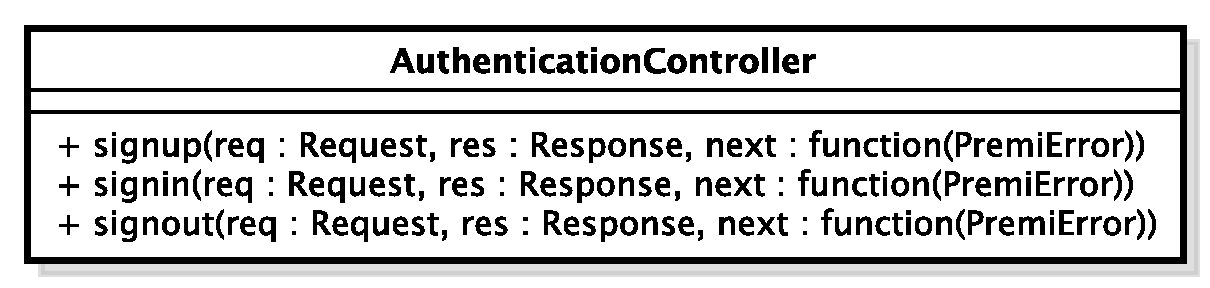
\includegraphics[scale=0.4,keepaspectratio]{diagrammi/classi/{BackEnd/App/Controllers/Users/authenticationCtlr}.pdf}}
\caption{\nogloxy{Premi::Back-End::App::Controllers::Users::AuthenticationController}}
\end{figure}
\FloatBarrier
\begin{itemize}
\item \textbf{Descrizione}\\
Classe che si occupa della registrazione e dell’autenticazione dell’utente nel sistema. \`E un componente ConcreteHandler del \gloxy{design pattern} Chain of responsibility. Risulta essere il componente che eventualmente esegue la richiesta del \gloxy{client} attraverso Passport.
\item \textbf{Utilizzo}\\
Viene utilizzata per implementare le funzionalità necessarie a gestire le richieste \gloxy{REST} legate alla registrazione e all'autenticazione dell'utente.
\item \textbf{Relazioni con altre classi}:
\begin{itemize}
\item \textit{IN} \hyperref[\nogloxy{Premi::Back-End::App::Controllers::UserController}]{\nogloxy{\texttt{UserController}}}\\
Classe che raggruppa attraverso \texttt{require} i vari controllers responsabili delle operazioni legate alla gestione degli utenti.
Si è scelto di predisporre questo raggruppamento per facilitare l’introduzione di nuove funzionalità legate alla gestione degli utenti.
\item \textit{OUT} \hyperref[\nogloxy{Premi::Back-End::App::Models::Session}]{\nogloxy{\texttt{Session}}}\\
Classe che gestisce la sessione utente dell'applicazione. \textit{Non sono stati modellati attributi e metodi di questa classe in quanto viene inizializzata da Express ed utilizzata da Passport attraverso funzionalità interne ai due middleware.}
\item \textit{OUT} \hyperref[\nogloxy{Premi::Back-End::App::Models::UserModel}]{\nogloxy{\texttt{UserModel}}}\\
Classe che modella la creazione e la gestione dei dati utente.
\end{itemize}
\item \textbf{Metodi}:
\begin{itemize}
\item \nogloxy{\texttt{+ signin(req: Request, res: Response, next: function(PremiError))}}
\\ Esegue l'autenticazione attraverso Passport, aggiorna i dati della sessione e risponde al \gloxy{client} con i dati non sensibili dell'utente che ha effettuato l'autenticazione.
\\ \textbf{Parametri}:
\begin{itemize}
\item \nogloxy{\texttt{req: Request}}
\\ Rappresenta la richiesta inviata dal \gloxy{client}, contiene la richiesta di login dell’utente.
\item \nogloxy{\texttt{res: Response}}
\\ Rappresenta la risposta che il \gloxy{server} fornirà al termine dell’esecuzione del metodo.
\item \nogloxy{\texttt{next: function(PremiError)}}
\\ \dpNext
\end{itemize}
\item \nogloxy{\texttt{+ signout(req: Request, res: Response)}}
\\ Esegue il logout dell'utente dal sistema.
\\ \textbf{Parametri}:
\begin{itemize}
\item \nogloxy{\texttt{req: Request}}
\\ Rappresenta la richiesta inviata dal \gloxy{client}, contiene la richiesta di logout inviata dal \gloxy{client}.
\item \nogloxy{\texttt{res: Response}}
\\ Rappresenta la risposta che il \gloxy{server} fornirà al termine dell’esecuzione del metodo.
\end{itemize}
\item \nogloxy{\texttt{+ signup(req: Request, res: Response, next: function(PremiError))}}
\\ Effettua la registrazione dell’utente nel sistema creando ed inserendo un nuovo document all’interno della collection \texttt{User}.
\\ \textbf{Parametri}:
\begin{itemize}
\item \nogloxy{\texttt{req: Request}}
\\ Rappresenta la richiesta inviata dal \gloxy{client}, contiene i dati che vengono inseriti nel nuovo document della collection \texttt{User} se tutti i campi dati del nuovo oggetto document creato sono corretti, altrimenti viene attivata la catena di gestione dell'errore.
\item \nogloxy{\texttt{res: Response}}
\\ Rappresenta la risposta che il \gloxy{server} fornirà al termine dell’esecuzione del metodo,contiene le informazioni non sensibili che l’utente ha inserito nel database e con cui viene identificato oppure contiene un messaggio d’errore.
\item \nogloxy{\texttt{next: function(PremiError)}}
\\ \dpNext
\end{itemize}
\end{itemize}
\end{itemize}
\subsubsubsection{\nogloxy{Premi::Back-End::App::Controllers::Users::AuthorizationController}}
\label{\nogloxy{Premi::Back-End::App::Controllers::Users::AuthorizationController}}
\begin{figure}[h]
\centering
\nogloxy{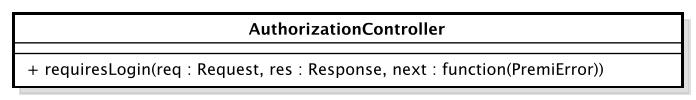
\includegraphics[scale=0.4,keepaspectratio]{diagrammi/classi/{BackEnd/App/Controllers/Users/authorizationCtrl}.pdf}}
\caption{\nogloxy{Premi::Back-End::App::Controllers::Users::AuthorizationController}}
\end{figure}
\FloatBarrier
\begin{itemize}
\item \textbf{Descrizione}\\
Classe middleware che, utilizzando Passport, si occupa di controllare la consistenza dell'oggetto \texttt{session} durante la sessione associata all'utente autenticato.  \`E un componente ConcreteHandler del \gloxy{design pattern} Chain of responsibility.
\item \textbf{Utilizzo}\\
Componente middleware della catena, esegue controlli sullo stato della sessione relativa all'utente. Se l'utente non possiede i permessi adeguati o la sessione è scaduta restituisce un messaggio d'errore, altrimenti passa il controllo al prossimo ConcreteHandler che gestirà il normale flusso d'esecuzione del programma.
\item \textbf{Relazioni con altre classi}:
\begin{itemize}
\item \textit{IN} \hyperref[\nogloxy{Premi::Back-End::App::Controllers::UserController}]{\nogloxy{\texttt{UserController}}}\\
Classe che raggruppa attraverso \texttt{require} i vari controllers responsabili delle operazioni legate alla gestione degli utenti.
Si è scelto di predisporre questo raggruppamento per facilitare l’introduzione di nuove funzionalità legate alla gestione degli utenti.
\item \textit{OUT} \hyperref[\nogloxy{Premi::Back-End::App::Models::Session}]{\nogloxy{\texttt{Session}}}\\
Classe che gestisce la sessione utente dell'applicazione. \textit{Non sono stati modellati attributi e metodi di questa classe in quanto viene inizializzata da Express ed utilizzata da Passport attraverso funzionalità interne ai due middleware.}
\item \textit{OUT} \hyperref[\nogloxy{Premi::Back-End::App::Models::UserModel}]{\nogloxy{\texttt{UserModel}}}\\
Classe che modella la creazione e la gestione dei dati utente.
\end{itemize}
\item \textbf{Metodi}:
\begin{itemize}
\item \nogloxy{\texttt{+ requiresLogin(req: Request, res: Response, next: function(PremiError))}}
\\ Metodo usato dal middleware per verificare che l'utente che esegue una richiesta sia effettivamente un utente autenticato.
\\ \textbf{Parametri}:
\begin{itemize}
\item \nogloxy{\texttt{req: Request}}
\\ Rappresenta la richiesta inviata dal \gloxy{client}.
\item \nogloxy{\texttt{res: Response}}
\\ Rappresenta la risposta che fornirà il \gloxy{server}.
\item \nogloxy{\texttt{next: function(PremiError)}}
\\ \dpNext
\end{itemize}
\end{itemize}
\end{itemize}
\subsection{\nogloxy{Premi::Back-End::App::Models}}
\label{\nogloxy{Premi::Back-End::App::Models}}
\subsubsection{Informazioni generali}
\begin{figure}[h]
\centering
\nogloxy{\includegraphics[scale=0.4,keepaspectratio]{diagrammi/package/{backEnd-app-models}.pdf}}
\caption{\nogloxy{Premi::Back-End::App::Models}}
\end{figure}
\FloatBarrier
\begin{itemize}
\item \textbf{Descrizione}\\
Package contenente le classi che definiscono il model dell'applicazione. Queste classi sono definite come classi schema di \gloxy{Mongoose}, il quale permette di utilizzare \gloxy{MongoDB} tramite degli oggetti.
\item \textbf{Padre}: \hyperref[\nogloxy{Premi::Back-End::App}]{\nogloxy{\texttt{App}}}
\end{itemize}
\subsubsection{Classi}
\subsubsubsection{\nogloxy{Premi::Back-End::App::Models::NodeContentModel}}
\label{\nogloxy{Premi::Back-End::App::Models::NodeContentModel}}
\begin{figure}[h]
\centering
\nogloxy{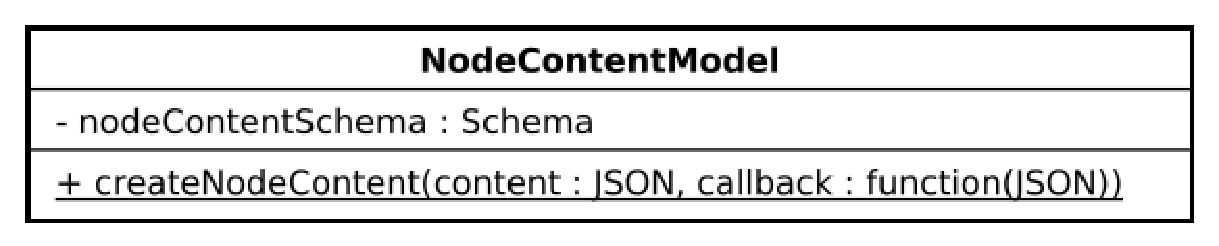
\includegraphics[scale=0.4,keepaspectratio]{diagrammi/classi/{BackEnd/App/Models/nodeContentModel}.pdf}}
\caption{\nogloxy{Premi::Back-End::App::Models::NodeContentModel}}
\end{figure}
\FloatBarrier
\begin{itemize}
\item \textbf{Descrizione}\\
Questa classe rappresenta gli elementi contenuti in un nodo della mappa mentale. Contiene le informazioni riguardanti la posizione e le dimensioni dell’oggetto all’interno del nodo.
\item \textbf{Utilizzo}\\
Viene utilizzata per rappresentare gli elementi contenuti in un nodo, distinguendo fra titolo, contenuto testuale e URL di un’immagine. Si interfaccia alla \gloxy{libreria} \gloxy{Mongoose} per la creazione dello schema e dei relativi metodi statici o di istanza.
\item \textbf{Relazioni con altre classi}:
\begin{itemize}
\item \textit{IN} \hyperref[\nogloxy{Premi::Back-End::App::Models::NodeModel}]{\nogloxy{\texttt{NodeModel}}}\\
Questa classe rappresenta i nodi della mappa mentale.
\end{itemize}
\item \textbf{Attributi}:
\begin{itemize}
\item \nogloxy{\texttt{- nodeContentSchema: Schema}}
\\ Questo campo dati rappresenta lo schema \gloxy{Mongoose} per il contenuto di un nodo e prevede i seguenti attributi:
\begin{itemize}
\item \texttt{content} di tipo \texttt{String}, rappresenta il contenuto di un elemento;
\item \texttt{x} di tipo \texttt{Number}, rappresenta la posizione sull’asse x di un elemento nel \gloxy{frame};
\item \texttt{y} di tipo \texttt{Number}, rappresenta la posizione sull’asse y di un elemento nel \gloxy{frame};
\item \texttt{height} di tipo \texttt{Number}, rappresenta l’altezza di un elemento nel \gloxy{frame};
\item \texttt{width} di tipo \texttt{Number}, rappresenta la larghezza di un elemento nel \gloxy{frame};
\item \texttt{class} di tipo \texttt{enum}, con tre possibili valori:
\begin{itemize}
\item \texttt{title};
\item \texttt{text};
\item \texttt{imgURL};
\end{itemize}
Questo attributo permette di capire il ruolo dell’elemento nel \gloxy{frame}.
\end{itemize}
\end{itemize}
\item \textbf{Metodi}:
\begin{itemize}
\item \nogloxy{\texttt{+ \uline{createNodeContent}(content: JSON, callback: function(JSON))}}
\\ Metodo statico che costruisce un nuovo elemento di contenuto. Restituisce un oggetto \gloxy{JSON} che descrive l’elemento.
\\ \textbf{Parametri}:
\begin{itemize}
\item \nogloxy{\texttt{content: JSON}}
\\ Rappresenta i dati del contenuto da utilizzare nella creazione.
\item \nogloxy{\texttt{callback: function(JSON)}}
\\ \dpCallback
\end{itemize}
\end{itemize}
\end{itemize}
\subsubsubsection{\nogloxy{Premi::Back-End::App::Models::NodeModel}}
\label{\nogloxy{Premi::Back-End::App::Models::NodeModel}}
\begin{figure}[h]
\centering
\nogloxy{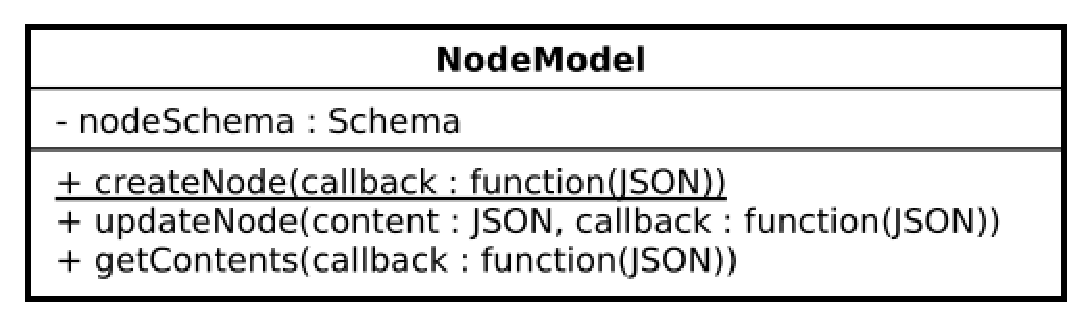
\includegraphics[scale=0.4,keepaspectratio]{diagrammi/classi/{BackEnd/App/Models/nodeModel}.pdf}}
\caption{\nogloxy{Premi::Back-End::App::Models::NodeModel}}
\end{figure}
\FloatBarrier
\begin{itemize}
\item \textbf{Descrizione}\\
Questa classe rappresenta i nodi della mappa mentale.
\item \textbf{Utilizzo}\\
Viene utilizzata per rappresentare i nodi di una mappa mentale. Si interfaccia alla \gloxy{libreria} \gloxy{Mongoose} per la creazione dello schema e dei relativi metodi statici o di istanza.
\item \textbf{Relazioni con altre classi}:
\begin{itemize}
\item \textit{IN} \hyperref[\nogloxy{Premi::Back-End::App::Models::PathModel}]{\nogloxy{\texttt{PathModel}}}\\
Questa classe rappresenta i \gloxy{percorsi di presentazione} eseguibili su una mappa mentale. Ogni \gloxy{percorso} è un aggregato dei nodi che l’utente vuole visualizzare nella presentazione.
\item \textit{IN} \hyperref[\nogloxy{Premi::Back-End::App::Models::ProjectModel}]{\nogloxy{\texttt{ProjectModel}}}\\
Questa classe rappresenta una mappa mentale, che contiene nodi, relazioni tra i nodi e \gloxy{percorsi} di presentazione.
\item \textit{IN} \hyperref[\nogloxy{Premi::Back-End::App::Models::RelationModel}]{\nogloxy{\texttt{RelationModel}}}\\
Questa classe rappresenta le relazioni tra i nodi di una mappa mentale. Ogni oggetto di tipo \texttt{RelationModel} modella il collegamento tra due nodi, di cui uno sarà individuato come sorgente della relazione e l’altro come destinazione. Le relazioni possono essere di due tipi, gerarchica (quando si vuole indicare che un nodo è figlio di un altro, come per un albero) oppure associazione.
\item \textit{OUT} \hyperref[\nogloxy{Premi::Back-End::App::Models::NodeContentModel}]{\nogloxy{\texttt{NodeContentModel}}}\\
Questa classe rappresenta gli elementi contenuti in un nodo della mappa mentale. Contiene le informazioni riguardanti la posizione e le dimensioni dell’oggetto all’interno del nodo.
\end{itemize}
\item \textbf{Attributi}:
\begin{itemize}
\item \nogloxy{\texttt{- nodeSchema: Schema}}
\\ Questo campo dati rappresenta lo schema \gloxy{Mongoose} per i nodi e prevede il seguente attributo:
\begin{itemize}
\item \texttt{content} di tipo \texttt{Array}, contiene oggetti di tipo \texttt{NodeContent}, che modellano i contenuti di un nodo. Essi devono essere trattati come subdocuments per \gloxy{Mongoose}.
\end{itemize}
\end{itemize}
\item \textbf{Metodi}:
\begin{itemize}
\item \nogloxy{\texttt{+ getContents(callback: function(JSON))}}
\\ Questo metodo restituisce un array di oggetti \gloxy{JSON} che rappresentano i contenuti di un nodo.
\\ \textbf{Parametri}:
\begin{itemize}
\item \nogloxy{\texttt{callback: function(JSON)}}
\\ \dpCallback
\end{itemize}
\item \nogloxy{\texttt{+ updateNode(content: JSON, callback: function(JSON))}}
\\ Questo metodo aggiorna i contenuti di un nodo. Restituisce un oggetto \gloxy{JSON} che descrive l’elemento dopo l’aggiornamento oppure un messaggio di errore.
\\ \textbf{Parametri}:
\begin{itemize}
\item \nogloxy{\texttt{content: JSON}}
\\ Rappresenta un array di contenuti da utilizzare per aggiornare i contenuti di un nodo.
\item \nogloxy{\texttt{callback: function(JSON)}}
\\ \dpCallback
\end{itemize}
\item \nogloxy{\texttt{+ \uline{createNode}(content: JSON, callback: function(JSON))}}
\\ Metodo statico che costruisce un nuovo nodo senza contenuti. Restituisce un oggetto \gloxy{JSON} che descrive l’elemento oppure un messaggio di errore.
\\ \textbf{Parametri}:
\begin{itemize}
\item \nogloxy{\texttt{content: JSON}}
\\ Rappresenta i dati del contenuto da utilizzare nella creazione.
\item \nogloxy{\texttt{callback: function(JSON)}}
\\ \dpCallback
\end{itemize}
\end{itemize}
\end{itemize}
\subsubsubsection{\nogloxy{Premi::Back-End::App::Models::PathModel}}
\label{\nogloxy{Premi::Back-End::App::Models::PathModel}}
\begin{figure}[h]
\centering
\nogloxy{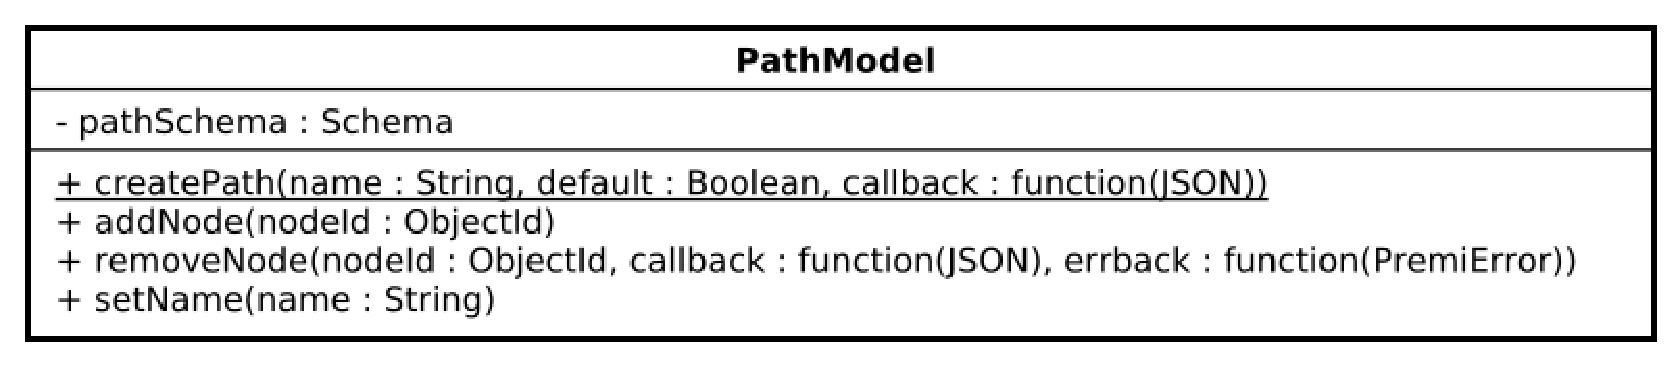
\includegraphics[scale=0.4,keepaspectratio]{diagrammi/classi/{BackEnd/App/Models/pathModel}.pdf}}
\caption{\nogloxy{Premi::Back-End::App::Models::PathModel}}
\end{figure}
\FloatBarrier
\begin{itemize}
\item \textbf{Descrizione}\\
Questa classe rappresenta i \gloxy{percorsi di presentazione} eseguibili su una mappa mentale. Ogni \gloxy{percorso} è un aggregato dei nodi che l’utente vuole visualizzare nella presentazione.
\item \textbf{Utilizzo}\\
Viene utilizzata per rappresentare i \gloxy{percorsi di presentazione} creabili ed eseguibili a partire da una mappa mentale. Si interfaccia alla \gloxy{libreria} \gloxy{Mongoose} per la creazione dello schema e dei relativi metodi statici o di istanza. Ogni \gloxy{progetto} ha sempre un \gloxy{percorso di presentazione} di default, che comprende tutti i nodi presenti nella mappa mentale, ordinati secondo l'ordine di creazione.
\item \textbf{Relazioni con altre classi}:
\begin{itemize}
\item \textit{IN} \hyperref[\nogloxy{Premi::Back-End::App::Models::ProjectModel}]{\nogloxy{\texttt{ProjectModel}}}\\
Questa classe rappresenta una mappa mentale, che contiene nodi, relazioni tra i nodi e \gloxy{percorsi} di presentazione.
\item \textit{OUT} \hyperref[\nogloxy{Premi::Back-End::App::Models::NodeModel}]{\nogloxy{\texttt{NodeModel}}}\\
Questa classe rappresenta i nodi della mappa mentale.
\end{itemize}
\item \textbf{Attributi}:
\begin{itemize}
\item \nogloxy{\texttt{- pathSchema: Schema}}
\\ Questo campo dati rappresenta lo schema \gloxy{Mongoose} per i \gloxy{percorsi di presentazione} e prevede i seguenti attributi:
\begin{itemize}
\item \texttt{nodes} di tipo \texttt{Array}, contiene gli \texttt{\gloxy{ObjectId}} dei nodi presenti in un \gloxy{percorso} di presentazione;
\item \texttt{name} di tipo \texttt{String}, rappresenta il nome che l’utente ha scelto per il \gloxy{percorso} di presentazione;
\item \texttt{default} di tipo \texttt{Boolean}, indica se il \gloxy{percorso} è quello di default per il \gloxy{progetto}.
\end{itemize}
\end{itemize}
\item \textbf{Metodi}:
\begin{itemize}
\item \nogloxy{\texttt{+ addNode(nodeId: ObjectId)}}
\\ Metodo che consente di aggiungere nodi al \gloxy{percorso} di presentazione.
\\ \textbf{Parametri}:
\begin{itemize}
\item \nogloxy{\texttt{nodeId: ObjectId}}
\\ Rappresenta l’identificativo del nodo nel database da aggiungere al \gloxy{percorso} di presentazione.
\end{itemize}
\item \nogloxy{\texttt{+ removeNode(nodeId: ObjectId, callback: function(JSON), errback: function(PremiError))}}
\\ Metodo che consente di rimuovere nodi dal \gloxy{percorso} di presentazione. Restituisce un oggetto \gloxy{JSON} che descrive l’elemento successivamente alla rimozione del nodo oppure un messaggio di errore.
\\ \textbf{Parametri}:
\begin{itemize}
\item \nogloxy{\texttt{nodeId: ObjectId}}
\\ Rappresenta l’identificativo del nodo nel database da rimuovere dal \gloxy{percorso} di presentazione.
\item \nogloxy{\texttt{callback: function(JSON)}}
\\ \dpCallback
\item \nogloxy{\texttt{errback: function(PremiError)}}
\\ \dpErrBack
\end{itemize}
\item \nogloxy{\texttt{+ setName(name: String)}}
\\ Metodo che consente di modificare il nome del \gloxy{percorso} di presentazione.
\\ \textbf{Parametri}:
\begin{itemize}
\item \nogloxy{\texttt{name: String}}
\\ Rappresenta il nuovo nome del \gloxy{percorso} di presentazione.
\end{itemize}
\item \nogloxy{\texttt{+ \uline{createPath}(name: String, default: Boolean, callback: function(JSON))}}
\\ Metodo statico che costruisce un nuovo \gloxy{percorso} inizialmente privo di nodi. Restituisce un oggetto \gloxy{JSON} che descrive l’elemento.
\\ \textbf{Parametri}:
\begin{itemize}
\item \nogloxy{\texttt{name: String}}
\\ Rappresenta il nome del \gloxy{percorso} che si vuole creare.
\item \nogloxy{\texttt{default: Boolean}}
\\ Specifica se il \gloxy{percorso} che da creare è quello di default.
\item \nogloxy{\texttt{callback: function(JSON)}}
\\ \dpCallback
\end{itemize}
\end{itemize}
\end{itemize}
\subsubsubsection{\nogloxy{Premi::Back-End::App::Models::ProjectModel}}
\label{\nogloxy{Premi::Back-End::App::Models::ProjectModel}}
\begin{figure}[h]
\centering
\nogloxy{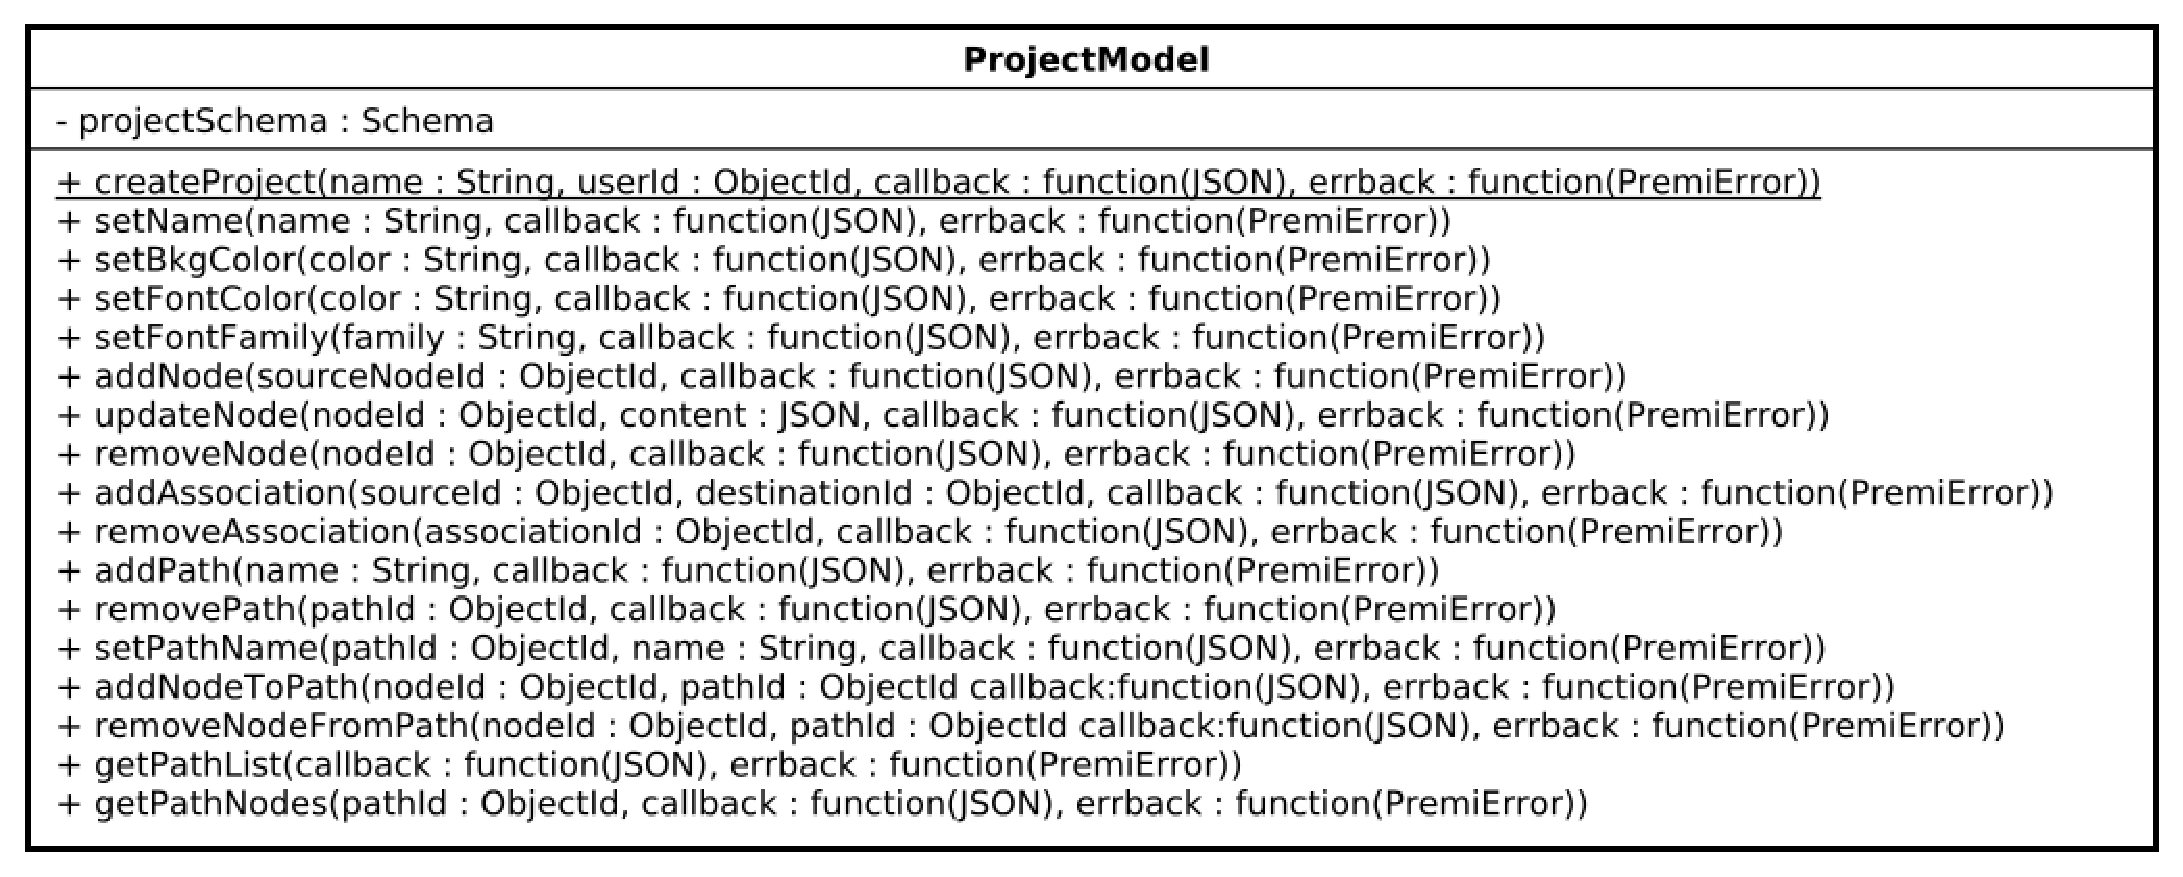
\includegraphics[scale=0.4,keepaspectratio]{diagrammi/classi/{BackEnd/App/Models/projectModel}.pdf}}
\caption{\nogloxy{Premi::Back-End::App::Models::ProjectModel}}
\end{figure}
\FloatBarrier
\begin{itemize}
\item \textbf{Descrizione}\\
Questa classe rappresenta una mappa mentale, che contiene nodi, relazioni tra i nodi e \gloxy{percorsi} di presentazione.
\item \textbf{Utilizzo}\\
Viene utilizzata per rappresentare una mappa mentale. Si interfaccia alla \gloxy{libreria} \gloxy{Mongoose} per la creazione dello schema e dei relativi metodi statici o di istanza. Questa classe implementa il \gloxy{design pattern} Façade e consente ai \gloxy{controller} di interagire con le classi del model che realizzano il \gloxy{progetto} attraverso la sua interfaccia pubblica.
\item \textbf{Relazioni con altre classi}:
\begin{itemize}
\item \textit{IN} \hyperref[\nogloxy{Premi::Back-End::App::Controllers::Projects::NodeController}]{\nogloxy{\texttt{NodeController}}}\\
Classe che gestisce la logica applicativa riguardante la visualizzazione e la modifica dei nodi presenti in un \gloxy{progetto}.
\item \textit{IN} \hyperref[\nogloxy{Premi::Back-End::App::Controllers::Projects::PathController}]{\nogloxy{\texttt{PathController}}}\\
Classe che gestisce la logica applicativa riguardante la visualizzazione e la modifica dei \gloxy{percorsi di presentazione} di un \gloxy{progetto}.
\item \textit{IN} \hyperref[\nogloxy{Premi::Back-End::App::Controllers::Projects::ProjectManagementController}]{\nogloxy{\texttt{ProjectManagementController}}}\\
Classe che gestisce la logica applicativa riguardante la visualizzazione e la modifica dei \gloxy{progetti}. Rappresenta il ConcreteHandler nel \gloxy{design pattern} Chain of responsibility. Utilizza Passport.
\item \textit{IN} \hyperref[\nogloxy{Premi::Back-End::App::Models::UserModel}]{\nogloxy{\texttt{UserModel}}}\\
Classe che modella la creazione e la gestione dei dati utente.
\item \textit{OUT} \hyperref[\nogloxy{Premi::Back-End::App::Models::NodeModel}]{\nogloxy{\texttt{NodeModel}}}\\
Questa classe rappresenta i nodi della mappa mentale.
\item \textit{OUT} \hyperref[\nogloxy{Premi::Back-End::App::Models::PathModel}]{\nogloxy{\texttt{PathModel}}}\\
Questa classe rappresenta i \gloxy{percorsi di presentazione} eseguibili su una mappa mentale. Ogni \gloxy{percorso} è un aggregato dei nodi che l’utente vuole visualizzare nella presentazione.
\item \textit{OUT} \hyperref[\nogloxy{Premi::Back-End::App::Models::RelationModel}]{\nogloxy{\texttt{RelationModel}}}\\
Questa classe rappresenta le relazioni tra i nodi di una mappa mentale. Ogni oggetto di tipo \texttt{RelationModel} modella il collegamento tra due nodi, di cui uno sarà individuato come sorgente della relazione e l’altro come destinazione. Le relazioni possono essere di due tipi, gerarchica (quando si vuole indicare che un nodo è figlio di un altro, come per un albero) oppure associazione.
\end{itemize}
\item \textbf{Attributi}:
\begin{itemize}
\item \nogloxy{\texttt{- projectSchema: Schema}}
\\ Questo campo dati rappresenta lo schema \gloxy{Mongoose} per i \gloxy{progetti} e prevede i seguenti attributi:
\begin{itemize}
\item \texttt{nodes} di tipo \texttt{Array}, contiene oggetti di tipo \texttt{Node} che devono essere trattati come subdocuments per \gloxy{Mongoose}
\item \texttt{root} di tipo \texttt{\gloxy{ObjectId}}, rappresenta il riferimento all'identificativo del nodo radice della mappa mentale;
\item \texttt{relations} di tipo \texttt{Array}, contiene oggetti di tipo \texttt{Relation} che devono essere trattati come subdocuments per \gloxy{Mongoose};
\item \texttt{paths} di tipo \texttt{Array}, contiene oggetti di tipo \texttt{Path} che devono essere trattati come subdocuments per \gloxy{Mongoose};
\item \texttt{name} di tipo \texttt{String}, rappresenta il nome che l’utente ha scelto per il \gloxy{progetto};
\item \texttt{userId} di tipo \texttt{\gloxy{ObjectId}}, rappresenta il riferimento all’identificativo nel database dell’utente proprietario del \gloxy{progetto};
\item \texttt{bkgColor} di tipo \texttt{String}, rappresenta il colore scelto per lo sfondo dei \gloxy{frame} in presentazione;
\item \texttt{fontColor} di tipo \texttt{String}, rappresenta il colore scelto per i testi nei \gloxy{frame} in presentazione;
\item \texttt{fontFamily} di tipo \texttt{String}, rappresenta la famiglia di font scelta per i testi nei \gloxy{frame} in presentazione.
\end{itemize}
\end{itemize}
\item \textbf{Metodi}:
\begin{itemize}
\item \nogloxy{\texttt{+ addAssociation(sourceId: ObjectId, destinationId: ObjectId, callback: function(JSON), errback: function(PremiError)): JSON}}
\\ Metodo  che costruisce una nuova relazione di tipo associazione. Restituisce un oggetto \gloxy{JSON} che descrive l’elemento oppure un messaggio di errore.
\\ \textbf{Parametri}:
\begin{itemize}
\item \nogloxy{\texttt{sourceId: ObjectId}}
\\ Rappresenta l'identificativo nel database del nodo sorgente della relazione.
\item \nogloxy{\texttt{destinationId: ObjectId}}
\\ Rappresenta l’identificativo nel database del nodo destinazione della relazione.
\item \nogloxy{\texttt{callback: function(JSON)}}
\\ \dpCallback
\item \nogloxy{\texttt{errback: function(PremiError)}}
\\ \dpErrBack
\end{itemize}
\item \nogloxy{\texttt{+ addNode(sourceNodeId: ObjectId, callback: function(JSON), errback: function(PremiError)): JSON}}
\\ Metodo che consente di aggiungere nodi vuoti al \gloxy{progetto} e quindi alla mappa mentale. Crea inoltre la relazione gerarchica tra il nuovo nodo e quello specificato come sorgente e lo aggiunge al \gloxy{percorso} di default. Restituisce un oggetto \gloxy{JSON} che descrive l'elemento aggiunto oppure un messaggio di errore.
\\ \textbf{Parametri}:
\begin{itemize}
\item \nogloxy{\texttt{sourceNodeId: ObjectId}}
\\ Rappresenta l'identificativo del nodo sorgente della relazione nel database.
\item \nogloxy{\texttt{callback: function(JSON)}}
\\ \dpCallback
\item \nogloxy{\texttt{errback: function(PremiError)}}
\\ \dpErrBack
\end{itemize}
\item \nogloxy{\texttt{+ addNodeToPath(nodeId: ObjectId, pathId: ObjectId, callback: function(JSON), errback: function(PremiError)): JSON}}
\\ Metodo che consente di aggiungere nodi ad un \gloxy{percorso} di presentazione. Restituisce un oggetto \gloxy{JSON} che descrive l’elemento oppure un messaggio di errore.
\\ \textbf{Parametri}:
\begin{itemize}
\item \nogloxy{\texttt{nodeId: ObjectId}}
\\ Rappresenta l'identificativo del nodo nel database, da aggiungere al \gloxy{percorso} di presentazione.
\item \nogloxy{\texttt{pathId: ObjectId}}
\\ Rappresenta l'identificativo del \gloxy{percorso} nel database a cui aggiungere il nodo.
\item \nogloxy{\texttt{callback: function(JSON)}}
\\ \dpCallback
\item \nogloxy{\texttt{errback: function(PremiError)}}
\\ \dpErrBack
\end{itemize}
\item \nogloxy{\texttt{+ addPath(pathId: ObjectId, callback: function(JSON), errback: function(PremiError)): JSON}}
\\ Metodo che consente di aggiungere un nuovo \gloxy{percorso di presentazione} con un nome specificato nei parametri. Restituisce un oggetto \gloxy{JSON} che descrive l’elemento oppure un messaggio di errore.
\\ \textbf{Parametri}:
\begin{itemize}
\item \nogloxy{\texttt{pathId: ObjectId}}
\\ Rappresenta l’identificativo del \gloxy{percorso} da rimuovere.
\item \nogloxy{\texttt{callback: function(JSON)}}
\\ \dpCallback
\item \nogloxy{\texttt{errback: function(PremiError)}}
\\ \dpErrBack
\end{itemize}
\item \nogloxy{\texttt{+ getPathList(callback: function(JSON), errback: function(PremiError)): JSON}}
\\ Metodo che consente di ottenere l’elenco dei \gloxy{percorsi di presentazione} del \gloxy{progetto}, ovvero un oggetto \gloxy{JSON} contenente coppie di identificativi e nomi dei \gloxy{percorsi}, attraverso la funzione di \gloxy{callback}.
\\ \textbf{Parametri}:
\begin{itemize}
\item \nogloxy{\texttt{callback: function(JSON)}}
\\ \dpCallback
\item \nogloxy{\texttt{errback: function(PremiError)}}
\\ \dpErrBack
\end{itemize}
\item \nogloxy{\texttt{+ getPathNodes(pathId: ObjectId, callback: function(JSON), errback: function(PremiError)): JSON}}
\\ Metodo che consente di ottenere l’elenco dei nodi presenti in un \gloxy{percorso di presentazione} del \gloxy{progetto} attraverso la funzione di \gloxy{callback}.
\\ \textbf{Parametri}:
\begin{itemize}
\item \nogloxy{\texttt{pathId: ObjectId}}
\\ Rappresenta l'identificativo nel database del \gloxy{percorso} di cui si vogliono ottenere i nodi.
\item \nogloxy{\texttt{callback: function(JSON)}}
\\ \dpCallback
\item \nogloxy{\texttt{errback: function(PremiError)}}
\\ \dpErrBack
\end{itemize}
\item \nogloxy{\texttt{+ removeAssociation(callback: function(JSON), errback: function(PremiError), associationId: ObjectId): JSON}}
\\ Metodo statico che rimuove un relazione di tipo \texttt{association}. Restituisce un oggetto \gloxy{JSON} che descrive l’elemento rimosso oppure un messaggio di errore.
\\ \textbf{Parametri}:
\begin{itemize}
\item \nogloxy{\texttt{callback: function(JSON)}}
\\ \dpCallback
\item \nogloxy{\texttt{errback: function(PremiError)}}
\\ \dpErrBack
\item \nogloxy{\texttt{associationId: ObjectId}}
\\ Rappresenta l'identificativo nel database dell'associazione da rimuovere.
\end{itemize}
\item \nogloxy{\texttt{+ removeNode(nodeId: ObjectId, callback: function(JSON), errback: function(PremiError)): JSON}}
\\ Metodo che consente di rimuovere nodi dal \gloxy{progetto} e quindi dalla mappa mentale. Se un nodo da rimuovere è radice di un sottoalbero, devono essere rimossi anche tutti i figli e le relazioni che coinvolgono il nodo. Deve aggiornare anche tutti i \gloxy{percorsi di presentazione} che contenevano quel nodo. Restituisce un oggetto \gloxy{JSON} che descrive la \gloxy{mappa mentale} priva del sottoalbero rimosso oppure un messaggio di errore.
\\ \textbf{Parametri}:
\begin{itemize}
\item \nogloxy{\texttt{nodeId: ObjectId}}
\\ Rappresenta l’identificativo del nodo nel database, da rimuovere.
\item \nogloxy{\texttt{callback: function(JSON)}}
\\ \dpCallback
\item \nogloxy{\texttt{errback: function(PremiError)}}
\\ \dpErrBack
\end{itemize}
\item \nogloxy{\texttt{+ removeNodeFromPath(nodeId: ObjectId, pathId: ObjectId, callback: function, errback: function(PremiError)): JSON}}
\\ Metodo che consente di rimuovere nodi da un \gloxy{percorso di presentazione} del \gloxy{progetto}. Restituisce un oggetto \gloxy{JSON} che descrive l’elemento oppure un messaggio di errore.
\\ \textbf{Parametri}:
\begin{itemize}
\item \nogloxy{\texttt{nodeId: ObjectId}}
\\ Questo parametro rappresenta l'identificativo del nodo nel database, da rimuovere dal \gloxy{percorso} di presentazione.
\item \nogloxy{\texttt{pathId: ObjectId}}
\\ Questo attributo rappresenta l'identificativo del \gloxy{percorso} nel database in cui rimuovere il nodo.
\item \nogloxy{\texttt{callback: function}}
\\ Questo parametro rappresenta la \gloxy{callback} che il metodo deve chiamare in caso di terminazione senza errori.
\item \nogloxy{\texttt{errback: function(PremiError)}}
\\ Questo parametro rappresenta la \gloxy{callback} che il metodo deve chiamare qualora si verificassero errori nell'esecuzione del metodo.
\end{itemize}
\item \nogloxy{\texttt{+ removePath(name: String, callback: function(JSON), errback: function(PremiError)): JSON}}
\\ Metodo che consente di rimuovere un \gloxy{percorso} di presentazione. Restituisce un oggetto \gloxy{JSON} che descrive l’elemento oppure un messaggio di errore.
\\ \textbf{Parametri}:
\begin{itemize}
\item \nogloxy{\texttt{name: String}}
\\ Rappresenta il nome del \gloxy{percorso} da rimuovere.
\item \nogloxy{\texttt{callback: function(JSON)}}
\\ \dpCallback
\item \nogloxy{\texttt{errback: function(PremiError)}}
\\ \dpErrBack
\end{itemize}
\item \nogloxy{\texttt{+ setBkgColor(color: String, callback: function(JSON), errback: function(PremiError)): JSON}}
\\ Metodo che consente di modificare il colore dello sfondo dei \gloxy{frame} in presentazione del \gloxy{progetto}. Restituisce un oggetto \gloxy{JSON} che descrive l’elemento oppure un messaggio di errore.
\\ \textbf{Parametri}:
\begin{itemize}
\item \nogloxy{\texttt{color: String}}
\\ Rappresenta il nome del colore di sfondo da impostare.
\item \nogloxy{\texttt{callback: function(JSON)}}
\\ \dpCallback
\item \nogloxy{\texttt{errback: function(PremiError)}}
\\ \dpErrBack
\end{itemize}
\item \nogloxy{\texttt{+ setFontColor(color: String, callback: function(JSON), errback: function(PremiError)): JSON}}
\\ Metodo che consente di modificare il colore dei testi dei \gloxy{frame} in presentazione del \gloxy{progetto}. Restituisce un oggetto \gloxy{JSON} che descrive l’elemento oppure un messaggio di errore.
\\ \textbf{Parametri}:
\begin{itemize}
\item \nogloxy{\texttt{color: String}}
\\ Rappresenta il colore da impostare come colore del testo.
\item \nogloxy{\texttt{callback: function(JSON)}}
\\ \dpCallback
\item \nogloxy{\texttt{errback: function(PremiError)}}
\\ \dpErrBack
\end{itemize}
\item \nogloxy{\texttt{+ setFontFamily(family: String, callback: function(JSON), errback: function(PremiError)): JSON}}
\\ Metodo che consente di modificare la famiglia di font dei testi dei \gloxy{frame} in presentazione del \gloxy{progetto}. Restituisce un oggetto \gloxy{JSON} che descrive l’elemento oppure un messaggio di errore.
\\ \textbf{Parametri}:
\begin{itemize}
\item \nogloxy{\texttt{family: String}}
\\ Rappresenta il nome della nuova famiglia di font per i testi del \gloxy{progetto}.
\item \nogloxy{\texttt{callback: function(JSON)}}
\\ \dpCallback
\item \nogloxy{\texttt{errback: function(PremiError)}}
\\ \dpErrBack
\end{itemize}
\item \nogloxy{\texttt{+ setName(name: String, callback: function(JSON), errback: function(PremiError)): JSON}}
\\ Metodo che consente di modificare il nome del \gloxy{progetto}. Restituisce un oggetto \gloxy{JSON} che descrive l’elemento oppure un messaggio di errore.
\\ \textbf{Parametri}:
\begin{itemize}
\item \nogloxy{\texttt{name: String}}
\\ Rappresenta il nuovo nome del \gloxy{progetto}.
\item \nogloxy{\texttt{callback: function(JSON)}}
\\ \dpCallback
\item \nogloxy{\texttt{errback: function(PremiError)}}
\\ \dpErrBack
\end{itemize}
\item \nogloxy{\texttt{+ setPathName(name: String, pathId: ObjectId, callback: function(JSON), errback: function(PremiError)): JSON}}
\\ Metodo che consente di modificare il nome di un \gloxy{percorso} di presentazione. Restituisce un oggetto \gloxy{JSON} che descrive l’elemento oppure un messaggio di errore.
\\ \textbf{Parametri}:
\begin{itemize}
\item \nogloxy{\texttt{name: String}}
\\ Rappresenta il nuovo nome del \gloxy{percorso} di presentazione.
\item \nogloxy{\texttt{pathId: ObjectId}}
\\ Rappresenta l'identificativo nel database del \gloxy{percorso} di cui si vuole modificare il nome.
\item \nogloxy{\texttt{callback: function(JSON)}}
\\ \dpCallback
\item \nogloxy{\texttt{errback: function(PremiError)}}
\\ \dpErrBack
\end{itemize}
\item \nogloxy{\texttt{+ updateNode(nodeId: ObjectId, content: JSON, callback: function(JSON), errback: function(PremiError)): JSON}}
\\ Metodo che consente di modificare il contenuto di un nodo nella mappa mentale.
\\ \textbf{Parametri}:
\begin{itemize}
\item \nogloxy{\texttt{nodeId: ObjectId}}
\\ Rappresenta l’identificativo del nodo da modificare.
\item \nogloxy{\texttt{content: JSON}}
\\ Rappresenta un array di oggetti \gloxy{JSON} con cui aggiornare il contenuto di un nodo. I contenuti precedenti vengono sovrascritti.
\item \nogloxy{\texttt{callback: function(JSON)}}
\\ \dpCallback
\item \nogloxy{\texttt{errback: function(PremiError)}}
\\ \dpErrBack
\end{itemize}
\item \nogloxy{\texttt{+ \uline{createProject}(name: String, userId: ObjectId, callback: function(JSON), errback: function(PremiError)): JSON}}
\\ Metodo statico che costruisce un nuovo \gloxy{progetto} che conterrà il primo nodo vuoto della mappa mentale.  Verrà inoltre istanziato il \gloxy{percorso} di default. Restituisce un oggetto \gloxy{JSON} che descrive l’elemento oppure un messaggio di errore.
\\ \textbf{Parametri}:
\begin{itemize}
\item \nogloxy{\texttt{name: String}}
\\ Rappresenta il nome del \gloxy{progetto} che si vuole creare.
\item \nogloxy{\texttt{userId: ObjectId}}
\\ Rappresenta l'id dell'utente che ha creato il \gloxy{progetto}.
\item \nogloxy{\texttt{callback: function(JSON)}}
\\ \dpCallback
\item \nogloxy{\texttt{errback: function(PremiError)}}
\\ \dpErrBackConstructor
\end{itemize}
\end{itemize}
\end{itemize}
\subsubsubsection{\nogloxy{Premi::Back-End::App::Models::RelationModel}}
\label{\nogloxy{Premi::Back-End::App::Models::RelationModel}}
\begin{figure}[h]
\centering
\nogloxy{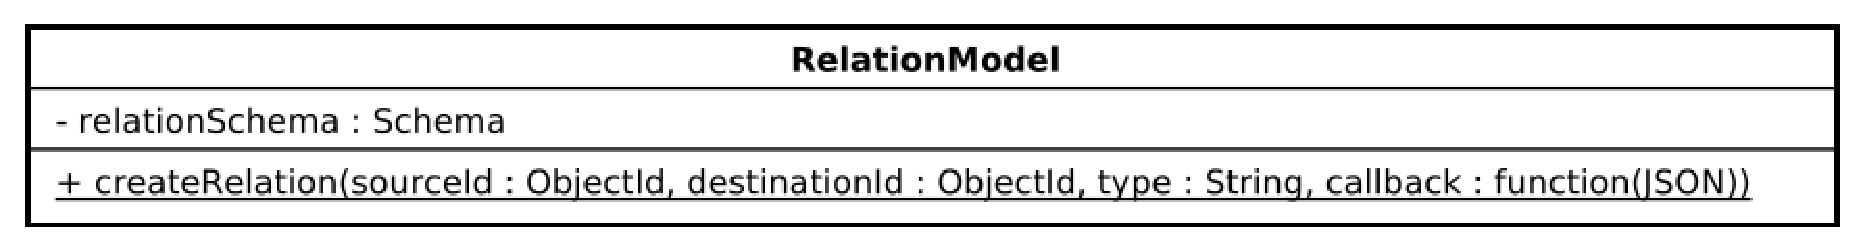
\includegraphics[scale=0.4,keepaspectratio]{diagrammi/classi/{BackEnd/App/Models/relationModel}.pdf}}
\caption{\nogloxy{Premi::Back-End::App::Models::RelationModel}}
\end{figure}
\FloatBarrier
\begin{itemize}
\item \textbf{Descrizione}\\
Questa classe rappresenta le relazioni tra i nodi di una mappa mentale. Ogni oggetto di tipo \texttt{RelationModel} modella il collegamento tra due nodi, di cui uno sarà individuato come sorgente della relazione e l’altro come destinazione. Le relazioni possono essere di due tipi, gerarchica (quando si vuole indicare che un nodo è figlio di un altro, come per un albero) oppure associazione.
\item \textbf{Utilizzo}\\
Viene utilizzata per rappresentare le relazione tra i nodi di una mappa mentale. Si interfaccia alla \gloxy{libreria} \gloxy{Mongoose} per la creazione dello schema e dei relativi metodi statici o di istanza.
\item \textbf{Relazioni con altre classi}:
\begin{itemize}
\item \textit{IN} \hyperref[\nogloxy{Premi::Back-End::App::Models::ProjectModel}]{\nogloxy{\texttt{ProjectModel}}}\\
Questa classe rappresenta una mappa mentale, che contiene nodi, relazioni tra i nodi e \gloxy{percorsi} di presentazione.
\item \textit{OUT} \hyperref[\nogloxy{Premi::Back-End::App::Models::NodeModel}]{\nogloxy{\texttt{NodeModel}}}\\
Questa classe rappresenta i nodi della mappa mentale.
\end{itemize}
\item \textbf{Attributi}:
\begin{itemize}
\item \nogloxy{\texttt{- relationSchema: Schema}}
\\ Questo campo dati rappresenta lo schema \gloxy{Mongoose} per le relazioni e prevede i seguenti attributi:
\begin{itemize}
\item \texttt{source} di tipo \texttt{\gloxy{ObjectId}}, rappresenta l’identificativo nel database del nodo sorgente della relazione;
\item \texttt{destination} di tipo \texttt{\gloxy{ObjectId}}, rappresenta l’identificativo nel database del nodo destinazione della relazione;
\item \texttt{class} di tipo enum, con due possibili valori:
\begin{itemize}
\item \texttt{hierarchical};
\item \texttt{association}.
\end{itemize}
Essi consentono di distinguere tra relazioni gerarchiche e associazioni.
\end{itemize}
\end{itemize}
\item \textbf{Metodi}:
\begin{itemize}
\item \nogloxy{\texttt{+ \uline{createRelation}(sourceId: ObjectId, destinationId: ObjectId, type: String, callback: function(JSON), errback: function(PremiError))}}
\\ Metodo statico che costruisce un nuova relazione. Restituisce un oggetto \gloxy{JSON} che descrive l’elemento oppure un messaggio di errore.
\\ \textbf{Parametri}:
\begin{itemize}
\item \nogloxy{\texttt{sourceId: ObjectId}}
\\ Rappresenta l’identificativo nel database del nodo sorgente della relazione.
\item \nogloxy{\texttt{destinationId: ObjectId}}
\\ Rappresenta l’identificativo nel database del nodo destinazione della relazione.
\item \nogloxy{\texttt{type: String}}
\\ Rappresenta il tipo di relazione che deve essere creata, scegliendo tra relazione gerarchica o associazione.
\item \nogloxy{\texttt{callback: function(JSON)}}
\\ \dpCallback
\item \nogloxy{\texttt{errback: function(PremiError)}}
\\ \dpErrBackConstructor
\end{itemize}
\end{itemize}
\end{itemize}
\subsubsubsection{\nogloxy{Premi::Back-End::App::Models::Session}}
\label{\nogloxy{Premi::Back-End::App::Models::Session}}
\begin{figure}[h]
\centering
\nogloxy{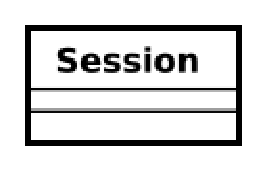
\includegraphics[scale=0.4,keepaspectratio]{diagrammi/classi/{BackEnd/App/Models/session}.pdf}}
\caption{\nogloxy{Premi::Back-End::App::Models::Session}}
\end{figure}
\FloatBarrier
\begin{itemize}
\item \textbf{Descrizione}\\
Classe che gestisce la sessione utente dell'applicazione. \textit{Non sono stati modellati attributi e metodi di questa classe in quanto viene inizializzata da Express ed utilizzata da Passport attraverso funzionalità interne ai due middleware.}
\item \textbf{Utilizzo}\\
Viene utilizzata da Passport per memorizzare i dati della sessione che viene creata quando un utente effettua il login.
\item \textbf{Relazioni con altre classi}:
\begin{itemize}
\item \textit{IN} \hyperref[\nogloxy{Premi::Back-End::App::Controllers::Users::AuthenticationController}]{\nogloxy{\texttt{AuthenticationController}}}\\
Classe che si occupa della registrazione e dell’autenticazione dell’utente nel sistema. \`E un componente ConcreteHandler del \gloxy{design pattern} Chain of responsibility. Risulta essere il componente che eventualmente esegue la richiesta del \gloxy{client} attraverso Passport.
\item \textit{IN} \hyperref[\nogloxy{Premi::Back-End::App::Controllers::Users::AuthorizationController}]{\nogloxy{\texttt{AuthorizationController}}}\\
Classe middleware che, utilizzando Passport, si occupa di controllare la consistenza dell'oggetto \texttt{session} durante la sessione associata all'utente autenticato.  \`E un componente ConcreteHandler del \gloxy{design pattern} Chain of responsibility.
\end{itemize}
\end{itemize}
\subsubsubsection{\nogloxy{Premi::Back-End::App::Models::UserModel}}
\label{\nogloxy{Premi::Back-End::App::Models::UserModel}}
\begin{figure}[h]
\centering
\nogloxy{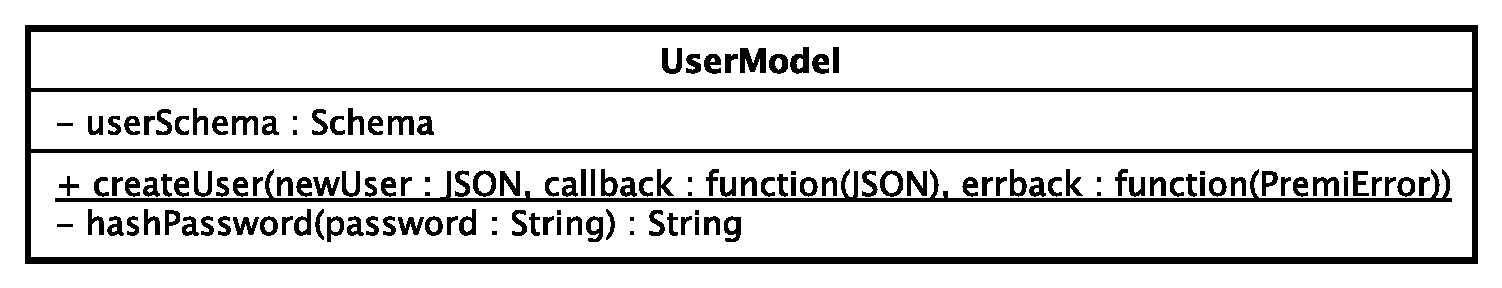
\includegraphics[scale=0.4,keepaspectratio]{diagrammi/classi/{BackEnd/App/Models/userModel}.pdf}}
\caption{\nogloxy{Premi::Back-End::App::Models::UserModel}}
\end{figure}
\FloatBarrier
\begin{itemize}
\item \textbf{Descrizione}\\
Classe che modella la creazione e la gestione dei dati utente.
\item \textbf{Utilizzo}\\
Viene utilizzata per rappresentare i dati degli account dei vari utenti dell'applicazione. Si interfaccia alla \gloxy{libreria} \gloxy{Mongoose} per la creazione dello schema e dei relativi metodi statici o di istanza.
\item \textbf{Relazioni con altre classi}:
\begin{itemize}
\item \textit{IN} \hyperref[\nogloxy{Premi::Back-End::App::Controllers::Users::AuthenticationController}]{\nogloxy{\texttt{AuthenticationController}}}\\
Classe che si occupa della registrazione e dell’autenticazione dell’utente nel sistema. \`E un componente ConcreteHandler del \gloxy{design pattern} Chain of responsibility. Risulta essere il componente che eventualmente esegue la richiesta del \gloxy{client} attraverso Passport.
\item \textit{IN} \hyperref[\nogloxy{Premi::Back-End::App::Controllers::Users::AuthorizationController}]{\nogloxy{\texttt{AuthorizationController}}}\\
Classe middleware che, utilizzando Passport, si occupa di controllare la consistenza dell'oggetto \texttt{session} durante la sessione associata all'utente autenticato.  \`E un componente ConcreteHandler del \gloxy{design pattern} Chain of responsibility.
\item \textit{OUT} \hyperref[\nogloxy{Premi::Back-End::App::Models::ProjectModel}]{\nogloxy{\texttt{ProjectModel}}}\\
Questa classe rappresenta una mappa mentale, che contiene nodi, relazioni tra i nodi e \gloxy{percorsi} di presentazione.
\end{itemize}
\item \textbf{Attributi}:
\begin{itemize}
\item \nogloxy{\texttt{- userSchema: Schema}}
\\ Questo campo dati rappresenta lo schema \gloxy{Mongoose} dell’utente Premi. Lo schema prevede i seguenti attributi:
\begin{itemize}
\item \texttt{username} di tipo \texttt{String}, rappresenta lo username con cui viene identificato l'utente all'interno dell'applicazione;
\item \texttt{password} di tipo \texttt{String}, rappresenta la password associata all'utente, viene dapprima concatenata con un campo dati \gloxy{salt} generato internamente da Passport e successivamente viene eseguito l'hashing;
\end{itemize}
\end{itemize}
\item \textbf{Metodi}:
\begin{itemize}
\item \nogloxy{\texttt{- hashPassword(password: String): String}}
\\ Effettua l'hashing della stringa \texttt{password} se non è già stata criptata tramite campo \texttt{\gloxy{salt}} per evitare attacchi di tipo \textit{rainbow}.
\\ \textbf{Parametri}:
\begin{itemize}
\item \nogloxy{\texttt{password: String}}
\\ Rappresenta la password dell'utente.
\end{itemize}
\item \nogloxy{\texttt{+ \uline{createUser}(newUser: JSON, callback: function(JSON), errback: function(PremiError))}}
\\ Metodo statico che costruisce un nuovo account associato ad un indirizzo e-mail.  Restituisce un oggetto \gloxy{JSON} che descrive l’elemento inserito oppure ritorna un messaggio di errore.
\\ \textbf{Parametri}:
\begin{itemize}
\item \nogloxy{\texttt{newUser: JSON}}
\\ Rappresenta i dati da utilizzare per la creazione di un nuovo utente.
\item \nogloxy{\texttt{callback: function(JSON)}}
\\ \dpCallback
\item \nogloxy{\texttt{errback: function(PremiError)}}
\\ \dpErrBackConstructor
\end{itemize}
\end{itemize}
\end{itemize}
\subsection{\nogloxy{Premi::Back-End::App::Routers}}
\label{\nogloxy{Premi::Back-End::App::Routers}}
\subsubsection{Informazioni generali}
\begin{figure}[h]
\centering
\nogloxy{\includegraphics[scale=0.4,keepaspectratio]{diagrammi/package/{backEnd-app-routers}.pdf}}
\caption{\nogloxy{Premi::Back-End::App::Routers}}
\end{figure}
\FloatBarrier
\begin{itemize}
\item \textbf{Descrizione}\\
Package contenente i router della componente \gloxy{back-end} dell’applicazione. Contiene i file di configurazione relativi al routing delle richieste del \gloxy{client}, ossia i routes di Express.
\item \textbf{Padre}: \hyperref[\nogloxy{Premi::Back-End::App}]{\nogloxy{\texttt{App}}}
\item \textbf{Interazioni con altri componenti}:
\begin{itemize}
\item \hyperref[\nogloxy{Premi::Back-End::App::Controllers}]{\nogloxy{\texttt{Controllers}}}\\
Package che contiene i controllers di Express, definisce la logica dell'applicazione.
\end{itemize}
\end{itemize}
\subsubsection{Classi}
\subsubsubsection{\nogloxy{Premi::Back-End::App::Routers::ProjectRouter}}
\label{\nogloxy{Premi::Back-End::App::Routers::ProjectRouter}}
\begin{figure}[h]
\centering
\nogloxy{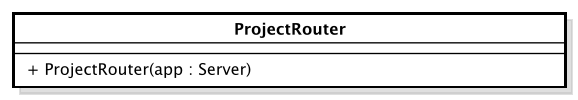
\includegraphics[scale=0.4,keepaspectratio]{diagrammi/classi/{BackEnd/App/Routers/projectRouter}.pdf}}
\caption{\nogloxy{Premi::Back-End::App::Routers::ProjectRouter}}
\end{figure}
\FloatBarrier
\begin{itemize}
\item \textbf{Descrizione}\\
Classe che gestisce le richieste relative alle operazioni riguardanti la mappa.  Componente ConcreteHandler del \gloxy{design pattern} Chain of responsibility.
\item \textbf{Utilizzo}\\
Viene utilizzata per chiamare il \gloxy{controller} che si occupa di gestire le \gloxy{API} relative alla mappa.
\item \textbf{Relazioni con altre classi}:
\begin{itemize}
\item \textit{IN} \hyperref[\nogloxy{Premi::Back-End::Server}]{\nogloxy{\texttt{Server}}}\\
Classe che avvia il \gloxy{server}. Nello specifico apre una connessione al database tramite \gloxy{Mongoose}, invoca il middleware Express passando un riferimento al database \gloxy{MongoDB} come parametro in modo che possa configurarsi con esso, invoca il middleware Passport ed infine si mette in ascolto su una determinata porta. \`E il componente \gloxy{client} del \gloxy{design pattern} Chain of responsibility. Utilizza i moduli \gloxy{Mongoose}, Express, Passport e Chalk, quest’ultimo serve per definire lo stile dei tipi \texttt{String}.
\item \textit{OUT} \hyperref[\nogloxy{Premi::Back-End::App::Controllers::ErrorHandler}]{\nogloxy{\texttt{ErrorHandler}}}\\
Classe middleware per la gestione degli errori. Ritorna al \gloxy{client} un oggetto di tipo \texttt{Response} con stato HTTP 500 e descrizione dell'errore in formato \gloxy{JSON}. \`E un componente ConcreteHandler del \gloxy{design pattern} Chain of responsibility.
\item \textit{OUT} \hyperref[\nogloxy{Premi::Back-End::App::Controllers::NotFoundHandler}]{\nogloxy{\texttt{NotFoundHandler}}}\\
Classe che si occupa della gestione dell'errore di pagina non trovata. Componente
ConcreteHandler del \gloxy{design pattern} Chain of responsibility.
\item \textit{OUT} \hyperref[\nogloxy{Premi::Back-End::App::Controllers::ProjectController}]{\nogloxy{\texttt{ProjectController}}}\\
Classe che raggruppa i vari controllers responsabili delle operazioni riguardanti la \gloxy{mappa mentale} attraverso \texttt{require}.
\end{itemize}
\item \textbf{Metodi}:
\begin{itemize}
\item \nogloxy{\texttt{+ ProjectRouter(app: Server)}}
\\ Contiene diverse route che vengono configurate all'avvio del \gloxy{server}. Quest'ultime ricevono le richieste del \gloxy{client} e passano il controllo al ConcreteHandler successivo.
\\ \textbf{Parametri}:
\begin{itemize}
\item \nogloxy{\texttt{app: Server}}
\\ Rappresenta l'istanza del \gloxy{server} su cui configurare i route che mappano i controllers specifici.
\end{itemize}
\end{itemize}
\end{itemize}
\subsubsubsection{\nogloxy{Premi::Back-End::App::Routers::StaticRouter}}
\label{\nogloxy{Premi::Back-End::App::Routers::StaticRouter}}
\begin{figure}[h]
\centering
\nogloxy{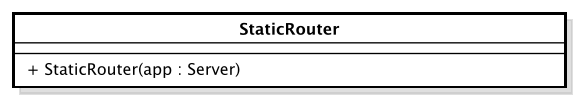
\includegraphics[scale=0.4,keepaspectratio]{diagrammi/classi/{BackEnd/App/Routers/staticRouter}.pdf}}
\caption{\nogloxy{Premi::Back-End::App::Routers::StaticRouter}}
\end{figure}
\FloatBarrier
\begin{itemize}
\item \textbf{Descrizione}\\
Classe che gestisce le richieste relative alle pagine statiche della componente \gloxy{back-end}. Componente ConcreteHandler del \gloxy{design pattern} Chain of responsibility.
\item \textbf{Utilizzo}\\
Viene utilizzata per fornire delle pagine \gloxy{HTML} statiche in risposta al \gloxy{client}, in particolare fornisce il manuale utente online.
\item \textbf{Relazioni con altre classi}:
\begin{itemize}
\item \textit{IN} \hyperref[\nogloxy{Premi::Back-End::Server}]{\nogloxy{\texttt{Server}}}\\
Classe che avvia il \gloxy{server}. Nello specifico apre una connessione al database tramite \gloxy{Mongoose}, invoca il middleware Express passando un riferimento al database \gloxy{MongoDB} come parametro in modo che possa configurarsi con esso, invoca il middleware Passport ed infine si mette in ascolto su una determinata porta. \`E il componente \gloxy{client} del \gloxy{design pattern} Chain of responsibility. Utilizza i moduli \gloxy{Mongoose}, Express, Passport e Chalk, quest’ultimo serve per definire lo stile dei tipi \texttt{String}.
\item \textit{OUT} \hyperref[\nogloxy{Premi::Back-End::App::Controllers::ErrorHandler}]{\nogloxy{\texttt{ErrorHandler}}}\\
Classe middleware per la gestione degli errori. Ritorna al \gloxy{client} un oggetto di tipo \texttt{Response} con stato HTTP 500 e descrizione dell'errore in formato \gloxy{JSON}. \`E un componente ConcreteHandler del \gloxy{design pattern} Chain of responsibility.
\item \textit{OUT} \hyperref[\nogloxy{Premi::Back-End::App::Controllers::NotFoundHandler}]{\nogloxy{\texttt{NotFoundHandler}}}\\
Classe che si occupa della gestione dell'errore di pagina non trovata. Componente
ConcreteHandler del \gloxy{design pattern} Chain of responsibility.
\item \textit{OUT} \hyperref[\nogloxy{Premi::Back-End::App::Controllers::StaticController}]{\nogloxy{\texttt{StaticController}}}\\
Classe che gestisce le operazioni e la logica applicativa riguardante la visualizzazione di pagine \gloxy{HTML} statiche. Rappresenta uno dei componenti ConcreteHandler del \gloxy{design pattern} Chain of responsibility.
\end{itemize}
\item \textbf{Metodi}:
\begin{itemize}
\item \nogloxy{\texttt{+ StaticRouter(app: Server)}}
\\ Contiene diverse route che vengono configurate all'avvio del \gloxy{server}. Quest'ultime ricevono le richieste del \gloxy{client} e passano il controllo al ConcreteHandler successivo.
\\ \textbf{Parametri}:
\begin{itemize}
\item \nogloxy{\texttt{app: Server}}
\\ Rappresenta l'istanza del \gloxy{server} su cui configurare i route che mappano i controllers specifici.
\end{itemize}
\end{itemize}
\end{itemize}
\subsubsubsection{\nogloxy{Premi::Back-End::App::Routers::UserRouter}}
\label{\nogloxy{Premi::Back-End::App::Routers::UserRouter}}
\begin{figure}[h]
\centering
\nogloxy{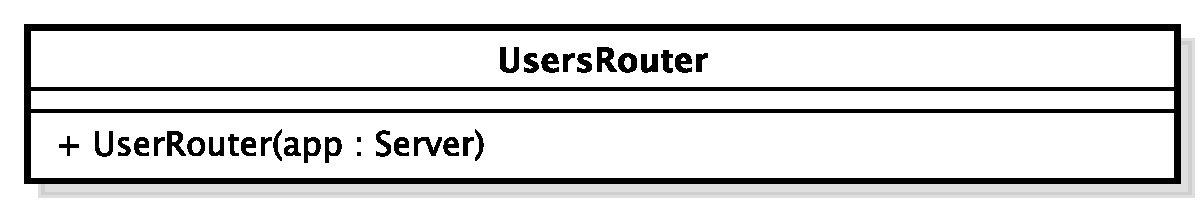
\includegraphics[scale=0.4,keepaspectratio]{diagrammi/classi/{BackEnd/App/Routers/userRouter}.pdf}}
\caption{\nogloxy{Premi::Back-End::App::Routers::UserRouter}}
\end{figure}
\FloatBarrier
\begin{itemize}
\item \textbf{Descrizione}\\
Classe che gestisce le richieste relative alla registrazione e alla gestione della sessione di un utente. Componente ConcreteHandler del \gloxy{design pattern} Chain of responsibility. Utilizza il modulo Passport.
\item \textbf{Utilizzo}\\
Viene utilizzata per chiamare il \gloxy{controller} che si occupa di gestire le \gloxy{API} relative alla registrazione e alla gestione della sessione di un utente.
\item \textbf{Relazioni con altre classi}:
\begin{itemize}
\item \textit{IN} \hyperref[\nogloxy{Premi::Back-End::Server}]{\nogloxy{\texttt{Server}}}\\
Classe che avvia il \gloxy{server}. Nello specifico apre una connessione al database tramite \gloxy{Mongoose}, invoca il middleware Express passando un riferimento al database \gloxy{MongoDB} come parametro in modo che possa configurarsi con esso, invoca il middleware Passport ed infine si mette in ascolto su una determinata porta. \`E il componente \gloxy{client} del \gloxy{design pattern} Chain of responsibility. Utilizza i moduli \gloxy{Mongoose}, Express, Passport e Chalk, quest’ultimo serve per definire lo stile dei tipi \texttt{String}.
\item \textit{OUT} \hyperref[\nogloxy{Premi::Back-End::App::Controllers::ErrorHandler}]{\nogloxy{\texttt{ErrorHandler}}}\\
Classe middleware per la gestione degli errori. Ritorna al \gloxy{client} un oggetto di tipo \texttt{Response} con stato HTTP 500 e descrizione dell'errore in formato \gloxy{JSON}. \`E un componente ConcreteHandler del \gloxy{design pattern} Chain of responsibility.
\item \textit{OUT} \hyperref[\nogloxy{Premi::Back-End::App::Controllers::NotFoundHandler}]{\nogloxy{\texttt{NotFoundHandler}}}\\
Classe che si occupa della gestione dell'errore di pagina non trovata. Componente
ConcreteHandler del \gloxy{design pattern} Chain of responsibility.
\item \textit{OUT} \hyperref[\nogloxy{Premi::Back-End::App::Controllers::UserController}]{\nogloxy{\texttt{UserController}}}\\
Classe che raggruppa attraverso \texttt{require} i vari controllers responsabili delle operazioni legate alla gestione degli utenti.
Si è scelto di predisporre questo raggruppamento per facilitare l’introduzione di nuove funzionalità legate alla gestione degli utenti.
\end{itemize}
\item \textbf{Metodi}:
\begin{itemize}
\item \nogloxy{\texttt{+ UserRouter(app: Server)}}
\\ Contiene diverse route che vengono configurate all'avvio del \gloxy{server}. Quest'ultime ricevono le richieste del \gloxy{client} e passano il controllo al ConcreteHandler successivo.
\\ \textbf{Parametri}:
\begin{itemize}
\item \nogloxy{\texttt{app: Server}}
\\ Rappresenta l'istanza del \gloxy{server} su cui configurare i route che mappano i controllers specifici.
\end{itemize}
\end{itemize}
\end{itemize}
\subsection{\nogloxy{Premi::Back-End::App::Views}}
\label{\nogloxy{Premi::Back-End::App::Views}}
\subsubsection{Informazioni generali}
\begin{figure}[h]
\centering
\nogloxy{\includegraphics[scale=0.4,keepaspectratio]{diagrammi/package/{backEnd-app-views}.pdf}}
\caption{\nogloxy{Premi::Back-End::App::Views}}
\end{figure}
\FloatBarrier
\begin{itemize}
\item \textbf{Descrizione}\\
Package contenente le views della componente \gloxy{back-end} dell’applicazione.
\item \textbf{Padre}: \hyperref[\nogloxy{Premi::Back-End::App}]{\nogloxy{\texttt{App}}}
\item \textbf{Interazioni con altri componenti}:
\begin{itemize}
\item \hyperref[\nogloxy{Premi::Back-End::App::Controllers}]{\nogloxy{\texttt{Controllers}}}\\
Package che contiene i controllers di Express, definisce la logica dell'applicazione.
\end{itemize}
\end{itemize}
\subsubsection{Classi}
\subsubsubsection{\nogloxy{Premi::Back-End::App::Views::UserManualView}}
\label{\nogloxy{Premi::Back-End::App::Views::UserManualView}}
\begin{figure}[h]
\centering
\nogloxy{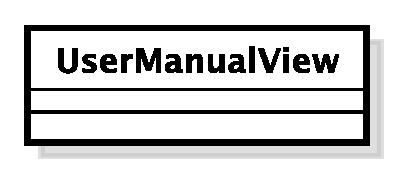
\includegraphics[scale=0.4,keepaspectratio]{diagrammi/classi/{BackEnd/App/Views/userManualView}.pdf}}
\caption{\nogloxy{Premi::Back-End::App::Views::UserManualView}}
\end{figure}
\FloatBarrier
\begin{itemize}
\item \textbf{Descrizione}\\
Pagina \gloxy{HTML} statica contenente il manuale dell’applicazione.
\item \textbf{Utilizzo}\\
Viene visualizzata quando l’utente richiede di consultare il manuale utente.
\item \textbf{Relazioni con altre classi}:
\begin{itemize}
\item \textit{IN} \hyperref[\nogloxy{Premi::Back-End::App::Controllers::StaticController}]{\nogloxy{\texttt{StaticController}}}\\
Classe che gestisce le operazioni e la logica applicativa riguardante la visualizzazione di pagine \gloxy{HTML} statiche. Rappresenta uno dei componenti ConcreteHandler del \gloxy{design pattern} Chain of responsibility.
\end{itemize}
\end{itemize}
\subsection{\nogloxy{Premi::Back-End::Config}}
\label{\nogloxy{Premi::Back-End::Config}}
\subsubsection{Informazioni generali}
\begin{figure}[h]
\centering
\nogloxy{\includegraphics[scale=0.4,keepaspectratio]{diagrammi/package/{backEnd-config}.pdf}}
\caption{\nogloxy{Premi::Back-End::Config}}
\end{figure}
\FloatBarrier
\begin{itemize}
\item \textbf{Descrizione}\\
Package contenente le componenti di configurazione del \gloxy{server}.
\item \textbf{Padre}: \hyperref[\nogloxy{Premi::Back-End}]{\nogloxy{\texttt{Back-End}}}
\item \textbf{Interazioni con altri componenti}:
\begin{itemize}
\item \hyperref[\nogloxy{Premi::Back-End::App}]{\nogloxy{\texttt{App}}}\\
Package contenente le componenti del \gloxy{server} che implementano il pattern \gloxy{MVC}.
\end{itemize}
\end{itemize}
\subsubsection{Classi}
\subsubsubsection{\nogloxy{Premi::Back-End::Config::Config}}
\label{\nogloxy{Premi::Back-End::Config::Config}}
\begin{figure}[h]
\centering
\nogloxy{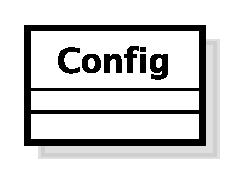
\includegraphics[scale=0.4,keepaspectratio]{diagrammi/classi/{BackEnd/Config/config}.pdf}}
\caption{\nogloxy{Premi::Back-End::Config::Config}}
\end{figure}
\FloatBarrier
\begin{itemize}
\item \textbf{Descrizione}\\
Questa classe gestisce la configurazione del \gloxy{server}. \textit{Non sono stati modellati attributi e metodi di questa classe in quanto viene gestita da Express.}
\item \textbf{Utilizzo}\\
Viene utilizzata per descrivere i parametri dell’applicazione. La classe \texttt{\gloxy{Server}} utilizza oggetti di questo tipo per creare ed avviare l’istanza del \gloxy{server}.
\item \textbf{Relazioni con altre classi}:
\begin{itemize}
\item \textit{IN} \hyperref[\nogloxy{Premi::Back-End::Server}]{\nogloxy{\texttt{Server}}}\\
Classe che avvia il \gloxy{server}. Nello specifico apre una connessione al database tramite \gloxy{Mongoose}, invoca il middleware Express passando un riferimento al database \gloxy{MongoDB} come parametro in modo che possa configurarsi con esso, invoca il middleware Passport ed infine si mette in ascolto su una determinata porta. \`E il componente \gloxy{client} del \gloxy{design pattern} Chain of responsibility. Utilizza i moduli \gloxy{Mongoose}, Express, Passport e Chalk, quest’ultimo serve per definire lo stile dei tipi \texttt{String}.
\end{itemize}
\end{itemize}
